\documentclass[journal]{IEEEtran}
\usepackage[T1]{fontenc}
\usepackage{amsmath, amssymb, xcolor, graphicx, comment, algorithm, algpseudocode}
\usepackage{multirow}
\usepackage{tikz}
\usetikzlibrary{arrows.meta, positioning}
\usepackage{soul}
\usepackage{placeins}   % \FloatBarrier to keep floats within their section
% Relax LaTeX's conservative float limits so figures are not deferred to a
% dedicated float page (helps figures sit near the referencing text).
\renewcommand{\topfraction}{0.92}
\renewcommand{\bottomfraction}{0.85}
\renewcommand{\textfraction}{0.07}
\renewcommand{\floatpagefraction}{0.75}
\setcounter{topnumber}{3}
\setcounter{bottomnumber}{2}
\setcounter{totalnumber}{5}
\DeclareMathOperator*{\argmax}{arg\,max}
\DeclareMathOperator*{\argmin}{arg\,min}
\DeclareMathOperator*{\sign}{\mbox{sign}}

\newcommand{\one}{\mathbf{1}}

\pagenumbering{arabic}

\usepackage{hyperref} 

\title{A Distributed Risk-Aware Bidding Strategy for Incorporating Renewable Generation and Dynamic Microgrids into Real-Time Electricity Market}
\author{\IEEEauthorblockN{Tommy Truong and Zhihua Qu
%\\\IEEEauthorblockA{University of Central Florida}
}
\thanks{The authors are with Department of Electrical and Computer Engineering, University of Central Florida, Orlando, FL 32816, USA. Emails: \href{mailto:to243763@ucf.edu}{to243763@ucf.edu} and 
\href{mailto:qu@ucf.edu}{qu@ucf.edu}.}}

\begin{document}

\maketitle

\begin{abstract}
This paper develops a coordinated design of risk aware bidding controllers for renewable operators and microgrid aggregators in day-ahead and real-time electricity markets. Each controller maximizes expected profit modified by a price-deviation term whose coefficient is prescribed before bidding. For fixed coefficients, the resulting bids form a Nash equilibrium of the controller objectives. In the uncapped model, we characterize the coefficient vectors for which this equilibrium attains the maximum aggregate expected profit of renewable operators; their sum must equal a negative constant when at least two operators participate. Equal risk seeking provides a symmetric coefficient design, whose bids are computed by masked consensus with a conditional privacy guarantee against passive collusion. A unilateral coefficient-deviation analysis shows that this design is not an equilibrium when owners independently select coefficients to maximize expected profit. The guarantees therefore concern coordinated controller design with assumed implementation, rather than incentive-compatible parameter selection. Illustrative cases compare the resulting expected-profit allocations.
\end{abstract}

%\begin{keywords}
{\it Keywords:} Risk-neutral and risk aware bidding strategies, Nash equilibrium, Pareto optimality, electricity markets, microgrids, distributed optimization, renewable energy
%\end{keywords}

\section{Introduction}

Competitive electricity markets operating under uncertainty exhibit a fundamental tension between individual rationality and collective efficiency. Renewable energy operators and/or their microgrid aggregators in particular face this challenge acutely: their generation is stochastic and correlated through shared weather conditions, their output forecasts are uncertain, and their bidding decisions must be submitted before real-time prices are known \cite{dvorkin2020chance, wong2007pricing, mieth2020distribution, 7930435}. When each operator optimizes its own expected profit independently, the resulting Nash equilibrium generally fails to achieve socially optimal outcomes,
even when all firms behave rationally \cite{zhang2016competition, lee2015rational, HobbsPang2007}.
This gap between Nash and Pareto-optimal performance is not merely a theoretical artifact: in markets with many correlated renewable operators, it translates directly into foregone collective profit and inefficient price signals \cite{asplund2002risk, wambach1999bertrand}.

Existing studies on stochastic Cournot and oligopoly games have examined the impact of uncertainty and risk preferences on equilibrium outcomes,
but they typically treat risk attitudes as fixed exogenous parameters and focus almost exclusively on risk averse firms \cite{cheng2002bertrand,sakai1989risk, gulpinar2014analysis, asplund2002risk, Chronopoulos2014}.
The same risk averse emphasis dominates bidding research in power markets, where conditional value-at-risk and related measures are used to shield generators, electric-vehicle aggregators, and virtual power plants from price volatility \cite{Barroso2009, Gong2009, Zheng2023, Xiao2025}.
Risk-seeking behavior, by contrast, is comparatively seldom modeled or systematically studied, and where optimism is considered it is posed as a behavioral trait rather than a controllable design variable \cite{Caraballo2015, Feng2023, ZhangEcon2020}; even recent risk sharing theory that admits risk seeking (convex) utilities treats the resulting equilibrium as descriptive rather than as an instrument a market operator can steer \cite{Lauzier2024}.
Those studies characterize equilibria conditional on preferences. Here we instead study coordinated design of controller coefficients; intrinsic preferences are not treated as freely adjustable actions. Separately, Pareto optimality has been studied through centralized optimization or cooperative formulations that require full information sharing \cite{hobbs2001individual, zhao2010social, su2018integrated}. These approaches are impractical in deregulated markets where operators are self-interested and unwilling to disclose private cost and forecast data. The most recent work~\cite{Truong26} starts the trend of bridging Nash equilibrium and Pareto optimality in the two-operator (duopoly) setting of Cournot game, but its outcome naturally yields with a risk averse strategy, in which each operator suppresses real-time price variability to protect its own payoff. Our present paper provides distinct results in two fundamentally different ways. First, it is shown that, in electricity markets, the gap between Nash equilibrium and the Pareto frontier is eliminated not by risk aversion but by a \emph{risk seeking} regime: the Pareto optimality requires a net negative constant on the sum of all market participants' risk level parameters, in the sense that the prescribed controller objectives reward price deviation rather than penalize it. Second, the analysis in the paper addresses electricity markets with $n$ renewable operators, and its uncapped equal risk seeking design admits distributed computation with a scoped privacy guarantee using established finite-field masking.

In parallel, stochastic and robust optimization models have been developed for microgrids and their aggregators to bid into day-ahead and real-time balancing markets \cite{7273948, 7393823, 8554122}, bi-level and tri-level formulations have been used to co-design retailer decisions and market operation \cite{9018247, 10908096}, and distributed schemes have been proposed for the energy management of multiple microgrids in real-time markets \cite{8141420}. However, in all of these formulations, each participant optimizes its own bid against exogenous prices or a fixed market design, nor have their distributed bid coordination been studied or Nash and Pareto properties been analyzed. 

We distinguish coordinated controller design from the subsequent bidding game. The participants jointly select the price-deviation coefficients to maximize aggregate expected renewable profit, and these coefficients remain fixed during bidding. Nash optimality then concerns each controller's bid under its prescribed objective. Implementation assumes adherence to the configured controllers; selecting the coefficients is not modeled as an equilibrium of self-interested owners. In particular, the coefficients are not declarations of intrinsic risk preferences, and their numerical computation does not establish commitment or incentive compatibility. Section~\ref{sec:beta_deviation} analyzes the distinct game in which owners may change their coefficients unilaterally. The proposed distributed algorithm computes the agreed design through neighboring communication \cite{qu, molzahn2017survey, yang2019survey}. This market-coordination layer connects microgrid aggregators through an overlaid communication network.


The remainder of the paper is organized as follows. Section~II formulates the day-ahead and real-time electricity markets in a stochastic setting and introduces risk aware objectives for renewable operators to perform cooperative and noncooperative optimization. In Section~III, coalition bidding strategy and Nash bidding strategy under fixed risk level parameters are derived, and potential overbidding in the risk neutral setting is studied. Section~IV characterizes coordinated controller designs, discusses bidding limits, and analyzes unilateral coefficient deviations. Section~V presents a distributed algorithm for renewable operators to implement their ERS strategies. Illustrative case studies are provided in Section~VI, followed by the concluding remarks in Section~VII.

\section{Problem Formulation}

In this paper, we consider the simple case that all traditional generation assets are owned by a single utility company\footnote{The proposed results apply to the general case of multiple utility companies of individual cost functions except for notational complexity.} while renewable generation is operated by individual entities (one of which could be the utility company). And the utility company and the renewable generation operators are the participants in both day-ahead and real-time electricity markets for profit. 

\begin{figure}[hbt!]
\centering
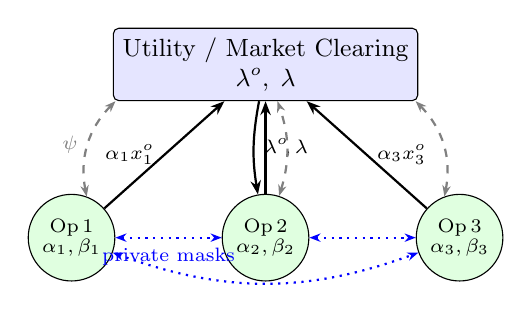
\begin{tikzpicture}[
  scale=0.88,
  mkt/.style={draw, rectangle, rounded corners=2pt, fill=blue!10,
              minimum width=3.4cm, minimum height=0.7cm,
              font=\small, align=center},
  op/.style={draw, circle, fill=green!12, minimum size=1.1cm,
             font=\scriptsize, align=center, inner sep=1pt},
  arr/.style={-{Stealth[length=5pt]}, thick},
  comm/.style={{Stealth[length=4pt]}-{Stealth[length=4pt]}, dashed, gray, thick}
]
\node[mkt] (util) at (0, 3.1) {Utility / Market Clearing\\$\lambda^o,\;\lambda$};
\node[op] (op1) at (-2.8, 0.6) {Op\,1\\[-1pt]$\alpha_1,\beta_1$};
\node[op] (op2) at (0,   0.6) {Op\,2\\[-1pt]$\alpha_2,\beta_2$};
\node[op] (op3) at ( 2.8, 0.6) {Op\,3\\[-1pt]$\alpha_3,\beta_3$};
% Bid submission
\draw[arr] (op1) -- node[left,  font=\scriptsize]{$\alpha_1 x_1^o$} (util);
\draw[arr] (op2) --                                                   (util);
\draw[arr] (op3) -- node[right, font=\scriptsize]{$\alpha_3 x_3^o$} (util);
% Price return
\draw[arr, bend right=10] (util) to
      node[right, font=\scriptsize]{$\lambda^o\!,\lambda$} (op2);
% Public consensus and separate private operator masking links
\draw[comm, bend left=28] (op1) to node[left, font=\scriptsize]{$\psi$} (util);
\draw[comm, bend right=18] (op2) to (util);
\draw[comm, bend right=28] (op3) to (util);
\draw[comm, blue, dotted] (op1) -- node[below, font=\scriptsize]{private masks} (op2);
\draw[comm, blue, dotted] (op2) -- (op3);
\draw[comm, blue, dotted, bend right=20] (op1) to (op3);
\end{tikzpicture}
\caption{Solid: submitted quantities and prices. Dashed: public consensus graph $G_c$. Dotted: private operator mask graph $G_m$. These are distinct logical communication layers.}
\label{fig:system_schematic}
\end{figure}

In an electricity market, utility aims to optimize a composite objective function in the form of 
\begin{equation} 
J(P_g) = a_2 P_g^2 + a_1 P_g + a_0, \label{eq:Jm}
\end{equation}
where $a_i$ are cost coefficients, and $P_g$ is the aggregated power of traditional generation. For simplicity, marginal costs of operating renewables and battery storage sites are modeled as zero, and hence they need not to be included explicitly in objective function \eqref{eq:Jm}. 

Let $n$ denote the total number of renewable generation operators and $\Omega=\{1,\cdots,n\}$ be the index set. For the day-ahead market, their renewable generations, $P_j$ for $j\in\Omega$, are modeled as stochastic variables, and similarly the grid total load $P_L$ is also modeled as a stochastic variable. Let us form the whole vector of random variables as 
\begin{equation} 
x = \begin{bmatrix} P_1 & \cdots & P_n & P_L \end{bmatrix}^T.  \label{eq:x}
\end{equation}
We assume that probability distribution of random vector $x$ is Gaussian as follows:
\[ f(x) = (2\pi)^{-\frac{n+1}{2}}\Sigma^{-\frac{1}{2}} e^{-\frac{1}{2}(x-x^o)^T\Sigma^{-1}(x-x^o)},  \]
where  $x^o=\mathbb{E}[x]$ is the vector of forecast (for the day-ahead market), and 
\begin{eqnarray*}
\Sigma & = & \mathbb{E}[(x-x^o)(x-x^o)^T] \\
& = & \begin{bmatrix} \sigma_{11} & \cdots & \sigma_{1n} & \sigma_{1L} \\ \vdots & \cdots & \vdots & \vdots \\ \sigma_{n1} & \cdots & \sigma_{nn} & \sigma_{nL} \\ \sigma_{1L} & \cdots & \sigma_{nL} & \sigma_{LL}
\end{bmatrix},  
\end{eqnarray*}
is the covariance matrix with $\sigma_{ij}=\sigma_{ji}$. In the covariance matrix, the last row and column correspond to covariances between the renewable generations and the load while $\sigma_{LL}=\sigma_L^2>0$ is the variance of the load. It is known that
$\sigma_{ii}=\sigma_i^2>0$, $\sigma_{ij}=\rho_{ij}\sigma_i\sigma_j$, $\sigma_{iL}=\rho_{iL}\sigma_i\sigma_L$, where $\rho_{ij},\rho_{iL}\in[0,1]$. Typically, $\rho_{ij},\rho_{iL}\not=0$ because renewable generations and load are correlated through the projected weather condition.

The Gaussian model is adopted for notational consistency with standard stochastic Cournot frameworks, but the key results of this paper require only that $x$ have finite mean $x^o$ and covariance $\Sigma$. The risk penalty $\mathbb{E}[(\lambda-\lambda^o)^2]$ and total profit $\Pi$ both expand as polynomials in the bidding coefficients with moment-based coefficients determined entirely by $x^o$ and $\Sigma$ (see~\eqref{eq:Pi_j_exp} and~\eqref{eq:sigma_lambda}), so Theorems~1--2 and Corollaries~1--5b hold for any joint distribution with finite second moments, including Weibull wind and beta solar distributions common in practice. Gaussianity would be needed only for distributional risk measures beyond variance (e.g., CVaR) or for characterizing higher moments of individual profits, which are deferred to future work.

The day-ahead market clears the projected aggregated power generation $P_g^o$ and its associated price $\lambda^o$ by minimizing $J(P_g^o)$ under the following power balance constraint:
\begin{equation} 
P_g^o + \sum_{j\in\Omega} \alpha_j x_j^o  = x_{n+1}^o, \label{eq:DA_power}
\end{equation}
where $x_{n+1}^o=P_L^o$, $\alpha_j\in[0,1]$ if no overbidding is allowed or $\alpha_j\in[0,\infty)$ if overbidding is permitted, and $\alpha_j x_j^o =\alpha_j P_j^o$ represent the bids by the renewable generation operators into the day-ahead market. Similarly, the real-time market clears the aggregated power generation $P_g$ and its associated price $\lambda$ by minimizing $J(P_g)$ under the following real-time power balance constraint:
\begin{equation} 
P_g + \sum_{j\in\Omega} x_j   = x_{n+1}. \label{eq:RT_power}
\end{equation}
It is well known that, with global information, day-ahead price $\lambda^o$ and real-time $\lambda$ are the dual variables associated with constraints \eqref{eq:DA_power} and \eqref{eq:RT_power}, respectively. 

The bidding controllers assigned to the renewable operators maximize the following objectives\footnote{Strictly speaking, we should use $J_i^{\prime} = \Pi_i - \beta_i \mathbb{E}[(\Pi_i - \mathbb{E}[\Pi_i])^2]$ which also yields a second-order polynomial in $\alpha_i$ as does \eqref{eq:J_i} but involves calculations of higher moments. Accordingly, \eqref{eq:J_i} is adopted instead.} individually:
\begin{subequations}
\begin{equation} 
J_i = \Pi_i - \beta_i \mathbb{E}[(\lambda - \lambda^o)^2], \label{eq:J_i}
\end{equation}
where $\beta_i\in\mathbb{R}$, 
\begin{equation} 
\Pi_i %= \lambda^o \alpha_i P_i^o + \mathbb{E}[\lambda (P_i - \alpha_i P_i^o)] 
= \lambda^o \alpha_i x_i^o + \mathbb{E}[\lambda (x_i - \alpha_i x_i^o)], \label{eq:Pi_i}
\end{equation}
\end{subequations}
Here $\alpha_i$ is the strategic action of controller $i$, whereas $\beta_i$ is a prescribed controller-design coefficient. We assume $a_2>0$ and $x_i^o>0$ for participating operators, and use $\beta_i\geq-1/(4a_2)$ in the Nash analysis. A positive coefficient penalizes the mean-square price deviation, a negative coefficient rewards it, and zero gives expected-profit maximization. The terms risk averse, risk seeking, and risk neutral describe these controller objectives, not the owners' intrinsic preferences.

For each fixed vector $\boldsymbol\beta$, the bidding game $G(\boldsymbol\beta)$ has payoffs $J_i$ and bid actions $\alpha_i$. Coefficients are selected jointly before the market interval and held fixed while controllers choose bids. We assume that participants implement the agreed controllers without unilateral coefficient changes or overrides of their generated bids during that interval. Such adherence requires a binding implementation arrangement; neither announcing coefficients nor running consensus establishes it. This paper assumes that arrangement and does not derive participation incentives or an enforcement mechanism.

The design criterion is the aggregate expected renewable profit $\Pi=\sum_i\Pi_i$ at the induced bidding equilibrium. Throughout, Nash optimality refers to the fixed controller objectives $J_i$, while Pareto efficiency refers to the expected-profit vector $(\Pi_1,\ldots,\Pi_n)$. Maximizing its sum establishes the latter, but does not establish Pareto efficiency in the $J_i$ utilities. Power grid congestion is outside the present model.

To characterize these strategies, we first solve the centralized case under global information, which provides the analytical foundation for the Nash equilibrium and Pareto conditions derived in subsequent sections.

\section{Centralized Risk-Aware Solution Under Global Information}

The electricity markets are bi-level optimization problems linked together by dual variables. At the upper level, they are quadratic optimization problems with equality constraints, that is, the markets perform their economic dispatch with the following Lagrangians: 
\begin{subequations}
\begin{equation} 
L^o = a_2(P_g^o)^2+a_1P_g^o+a_0 + \lambda^o\left(x_{n+1}^o- P_g^o-\sum_{j\in\Omega} \alpha_j x_j^o \right), \label{eq:L*}
\end{equation}
\begin{equation} 
L = a_2P_g^2+a_1P_g+a_0 + \lambda\left(x_{n+1}-P_g-\sum_{j\in\Omega} x_j\right). \label{eq:L}
\end{equation}
\end{subequations}
Applying the first-order optimality condition to the Lagrangians yields the following solutions for the prices:
\begin{subequations}
\begin{equation} 
\lambda^o = 2a_2P_g^o +a_1 = 2a_2\left(x_{n+1}^o-\sum_{j\in\Omega} \alpha_j x_j^o \right) +a_1 , \label{eq:lambda*}
\end{equation}
\begin{equation} 
\lambda = 2a_2P_g+a_1=2a_2\left(x_{n+1}-\sum_{j\in\Omega} x_j \right) + a_1. \label{eq:lambda}
\end{equation}
\end{subequations}

The lower-level optimization problems are also quadratic, and the centralized solutions under global information are summarized into the following lemma and theorem. Lemma 1 provides the solution of cooperative optimization when all the entities bind themselves together and act as one. In this case, the best outcome for the group is achieved under the risk neutral strategy.

\noindent \textbf{Lemma 1:} {\it Consider the case that all renewable generation entities form a coalition by sharing all the information and setting $\alpha_i=\alpha$ and $\beta_i=\frac{1}{n}\beta$, respectively. Then, for any choice of $\beta\in[-(4a_2)^{-1},\; +\infty)$, the optimal bidding strategy to optimize objective function $\sum_i J_i$ with $J_i$ in \eqref{eq:J_i} is
\begin{equation}
\alpha^* = \frac{1 + 4a_2 \beta}{2(1 + 2a_2\beta)}.
\label{eq:alpha_1}
\end{equation}
In addition, by further choosing $\beta_i$ to optimize $\sum_i \Pi_i$ with $\Pi_i$ in \eqref{eq:Pi_i}, the jointly designed coefficient and its induced coalition bid are}
\begin{equation}
\alpha^*  =  \frac{1}{2}, \quad
\beta^*  =  0.
\label{eq:optimal_1}
\end{equation}

\noindent \textbf{Proof:} It follows from \eqref{eq:Pi_i} and \eqref{eq:lambda*} that, if $\alpha_i=\alpha$, 
\begin{eqnarray*}
\Pi_r & = & \sum_{j\in\Omega} \Pi_j = \lambda^o \alpha x_r^o +  \mathbb{E}[\lambda (x_r-\alpha x_r^o)] \\
 \lambda^o   & = & 2a_2\left(x_{n+1}^o-\alpha x_r^o \right) +a_1,
\end{eqnarray*}
where $x_r = \sum_{j\in\Omega} x_j$ is the total renewable generation, and $x_r^o = \sum_{j\in\Omega} x_j^o$. Substituting \eqref{eq:lambda} into the above equations yields
\begin{eqnarray}
\Pi_r & = &  [2a_2\left(x_{n+1}^o-\alpha x_r^o \right) +a_1] \alpha x_r^o \nonumber \\
&& + \mathbb{E}[(2a_2\left(x_{n+1}-x_r \right) + a_1)(x_r-\alpha x_r^o)] \nonumber \\
  & = & 2a_2\alpha(1-\alpha)(x_r^o)^2 +a_1x_r^o  + 2a_2\mathbb{E}[\left(x_{n+1}x_r-x_r^2 \right)] \nonumber\\
   & = & 2a_2\alpha(1-\alpha)(x_r^o)^2 +a_1x_r^o \nonumber \\
   && + 2a_2\left(x_{n+1}^ox_r^o+\sigma_{rL}-(x_r^o)^2-\sigma_r^2 \right), \label{eq:Pi_r_exp}
\end{eqnarray}
where $\sigma_{rL}\triangleq\sum_{i\in\Omega}\sigma_{iL}$ is the total renewable-load cross-covariance, $\one$ is the $n$-dimensional column vector of $1$s, and
\begin{eqnarray*}
    \sigma_r^2 & = & \mathbb{E}[(x_1+\cdots+x_n-(x_1^o+\cdots+x_n^o))^2] \\
    & = & \mathbb{E}[ \one^T (x_r-x_r^o)(x_r-x_r^o)^T\one] \\
    & = & \one^T \Sigma_r \one \;=\; \sum_{i\in\Omega}\sum_{j\in\Omega} \sigma_{ij},
\end{eqnarray*}
where $x_r = [x_1,\cdots,x_n]^T$ is the $n$-vector of renewable generations and $\Sigma_r$ is the upper-left $n\times n$ subblock of $\Sigma$ containing only the renewable-to-renewable covariances $\sigma_{ij}$, $i,j\in\{1,\cdots,n\}$.
On the other hand it follows from \eqref{eq:J_i}, \eqref{eq:lambda*}, and \eqref{eq:lambda} that, if $\beta_i = \frac{1}{n}\beta$,
\begin{eqnarray*}
J_r & = & \sum_{j\in\Omega} J_j \\
 & = & \Pi_r  - \beta \mathbb{E}[2a_2 (x_{n+1}-x_{n+1}^o -x_r +\alpha x_r^o)^2] \\
 & = & 2a_2\alpha(1-\alpha)(x_r^o)^2  - 4a_2^2  \beta  (1-\alpha)^2 (x_r^o)^2 \\
 & & +a_1x_r^o + 2a_2\left(x_{n+1}^ox_r^o+\sigma_{rL}-(x_r^o)^2-\sigma_r^2 \right)\\
 && - 4a_2^2  \beta (\sigma_L^2+\sigma_r^2 - 2\sigma_{rL}). 
\end{eqnarray*}
Using the above expression, taking the partial derivative of $J_r$ with respect to $\alpha$, and setting the partial derivative to zero yield optimal bidding strategy \eqref{eq:alpha_1}. 

Substituting solution \eqref{eq:alpha_1} into 
\eqref{eq:Pi_r_exp} and differentiating $\Pi_r$ with respect to $\beta$ yields
\[ \frac{\partial \Pi_r}{\partial \beta} = - 2a_2(x_r^o)^2\frac{4a_2^2\beta}{(1+2a_2\beta)^3}, \]
which yields the optimal bidding strategy \eqref{eq:optimal_1}. This completes the proof. \hfill $\Box$

It follows from \eqref{eq:alpha_1} that
\[ \lim_{\beta\rightarrow-1/(4a_2)} \alpha = 0, \quad  \lim_{\beta\rightarrow0} \alpha = 0.5, \quad \lim_{\beta\rightarrow +\infty} \alpha = 1. \]
For the coalition, the prescribed coefficient $\beta$ determines the bid through~\eqref{eq:alpha_1}. The noncooperative bidding game below similarly depends on fixed controller coefficients, which are selected at a separate coordinated design stage.

The following theorem provides the solution to non-cooperative optimization in which each agent devises its strategy according to its own objective function $J_i$. 

\noindent \textbf{Theorem 1:} {\it Consider the uncapped bidding game with $a_2>0$ and $x_i^o>0$. For every fixed prescribed vector with $\beta_i\in[-(4a_2)^{-1},+\infty)$, the optimal bidding strategy $\alpha_i^*$ to optimize objective $J_i$ in \eqref{eq:J_i} forms a Nash equilibrium corresponding to the solution to the linear algebraic equation:
denoting $\boldsymbol{\alpha}^*=[\alpha_1^* \; \cdots \; \alpha_n^*]^T$,
\begin{equation}
A \boldsymbol{\alpha}^* = B,
\label{eq:alpha_i}
\end{equation}
where $x_r^o = \sum_{j\in\Omega} x_j^o$, $\eta_i = x_i^o/x_r^o\geq0$ with $\sum_{i\in\Omega} \eta_i=1$, and
\[ A=[A_{ij}], \quad A_{ij} = \left\{ \begin{array}{ll} 2(1+2a_2\beta_i)\eta_i & \mbox{if $i=j$} \\
(1+4a_2\beta_i)\eta_j & \mbox{if $i\not=j$}\end{array} \right., \]
and
\[ B=[B_i], \quad B_i = (1+4a_2\beta_i). \]
At the coordinated design stage, the total profit $\Pi=\sum_{i\in\Omega}\Pi_i$ can be maximized by jointly selecting $\boldsymbol\beta$ to maximize the following function:
\begin{equation} 
g(\boldsymbol{\alpha}^*) = f(\boldsymbol{\alpha}^*) \left[ 1 - f(\boldsymbol{\alpha}^*)  \right](x_r^o)^2,
\label{eq:G}
\end{equation} 
where  
\begin{equation} 
f(\boldsymbol{\alpha}) \stackrel{\triangle}{=} \sum_{i\in\Omega}  \alpha_i \eta_i.  
\label{eq:F}
\end{equation} 
}

\noindent \textbf{Proof:} It follows from \eqref{eq:Pi_i},  \eqref{eq:lambda*}, and \eqref{eq:lambda} that 
\begin{eqnarray}
\Pi_i & = & \left[ 2a_2\left(x_{n+1}^o-\sum_j \alpha_j x_j^o
  \right) +a_1 \right] \alpha_i x_i^o \nonumber \\ && 
  + \mathbb{E}\left[\left(2a_2\left(x_{n+1}-\sum_j x_j \right) + a_1\right) (x_i - \alpha_i x_i^o)\right] \nonumber \\
  & = & 2a_2\sum_j\alpha_i(1-\alpha_j)x_j^o x_i^o +a_1 x_i^o  \nonumber \\
  && + 2a_2\mathbb{E}\left[\left(x_{n+1}-\sum_j x_j \right) x_i\right] \nonumber\\
   & = & 2a_2\sum_j\alpha_i(1-\alpha_j)x_j^o x_i^o +a_1 x_i^o  \nonumber \\
  && + 2a_2\left(x_{n+1}^o x_i^o + \sigma_{iL}- \sum_j (x_j^o x_i^o+\sigma_{ij})\right), \label{eq:Pi_j_exp}
\end{eqnarray}
where the identity $\mathbb{E}[x_ix_j]=x_i^ox_j^o+\sigma_{ij}$ is used. On the other hand it follows from \eqref{eq:lambda*} and \eqref{eq:lambda} that 
\begin{eqnarray} 
&& \mathbb{E}[(\lambda - \lambda^o)^2] \nonumber \\
& = & 
4a_2^2  \mathbb{E}\left[\left(x_{n+1}-x_{n+1}^o -\sum_{j\in\Omega} (x_j-\alpha_j x_j^o)\right)^2\right] \nonumber \\
& = & 4a_2^2\left[\sigma_{LL} + 2\sum_{j\in\Omega} \sigma_{jL} + 2 \sum_{j\in\Omega} \sum_{l\in\Omega} \sigma_{jl} \right. \nonumber \\
&& \left.+ \left(\sum_{j\in\Omega} (1-\alpha_j) x_j^o\right)^2 \right]
, \label{eq:sigma_lambda}
\end{eqnarray}
The expression of $J_i$ defined in \eqref{eq:J_i} becomes explicit in terms of $\alpha_i$ by combining \eqref{eq:Pi_j_exp} and \eqref{eq:sigma_lambda}. Taking the partial derivatives of $J_i$ with respect to $\alpha_i$ yields
\begin{subequations}
\begin{eqnarray} 
\frac{\partial J_i}{\partial \alpha_i} & = &  2a_2(1+4a_2\beta_i) \sum_{j\in\Omega}(1-\alpha_j)x_j^o x_i^o \nonumber \\&& 
- 2a_2 \alpha_i (x_i^o)^2, \label{eq:p1_Ji} \\
\frac{\partial J^2_i}{\partial \alpha_i^2} & = & - 4a_2(1+2a_2\beta_i) (x_i^o)^2 <0 \;\;\; \forall \beta_i\geq-\frac{1}{4a_2}. \hspace*{.3in} \label{eq:p2_Ji}
\end{eqnarray}
\end{subequations}
Equation \eqref{eq:p2_Ji} shows that, for each fixed choice of the other players' bids, $J_i$ is strictly concave in $\alpha_i$. Hence any feasible stationary point is the unique best response of controller $i$. Setting \eqref{eq:p1_Ji} to zero yields
\begin{equation}
   (1+4a_2\beta_i) \sum_{j\in\Omega}(1-\alpha_j)x_j^o 
- \alpha_i x_i^o=0, \label{eq:p1Ji=0}
\end{equation}  
To include boundary bids, define $q_i=\alpha_i x_i^o$, $Q=\sum_iq_i$, and $k_i=1+4a_2\beta_i\geq0$. No equilibrium can have $Q\geq x_r^o$: by~\eqref{eq:p1_Ji}, any positive bidder would benefit from reducing its bid. Thus $Q<x_r^o$ at equilibrium. A controller with $k_i>0$ then bids positively, whereas $k_i=0$ gives $q_i=0$. All equilibrium bids therefore satisfy~\eqref{eq:p1Ji=0}.

Collecting these equations yields~\eqref{eq:alpha_i}. Writing $K=\sum_i k_i$, their sum gives $Q=Kx_r^o/(1+K)$ and then $q_i=k_ix_r^o/(1+K)$. This nonnegative solution is unique and satisfies each controller's best response.

It follows from \eqref{eq:alpha_i} that $\alpha_i^*$ are functions of $\beta_j$. We know from  \eqref{eq:Pi_j_exp} that 
\begin{eqnarray}
    \Pi & = & \sum_i \Pi_i \nonumber \\
     & = & 2a_2\left[ g(\boldsymbol{\alpha}) - \left(x_r^o\right)^2 + x_{n+1}^o x_r^o\right]  +a_1 x_r^o  \nonumber \\ 
     && + 2a_2 \left[ \sum_{i\in\Omega} \sigma_{iL} -\sum_{i\in\Omega}\sum_{j\in\Omega}\sigma_{ij}\right], \label{eq:Pi_exp}
\end{eqnarray}
where
\[ g(\boldsymbol{\alpha}) \stackrel{\triangle}{=} \sum_{i\in\Omega}  \alpha_i x_i^o  \sum_{j\in\Omega} (1-\alpha_j ) x_j^o. \]
Hence, $\Pi$ is maximized if function $g(\cdot)$ is maximized by choosing $\beta_j$.
Simplifying the above expression of $g(\cdot)$ yields \eqref{eq:G}. This completes the proof. \hfill $\Box$

Theorem 1 extends the results in \cite{Chow2017} in several ways. First, load uncertainties and correlations among the renewable generations are considered.  As a result, we know from \eqref{eq:Pi_exp} that the degradation of total profit function $\Pi$ due to uncertainties is 
\begin{equation} 
\Delta \Pi = 2a_2 \left[ \sum_{i\in\Omega}\sum_{j\in\Omega}\sigma_{ij}- \sum_{i\in\Omega} \sigma_{iL}\right], \label{eq:D_P}
\end{equation}
is less as long as there is some correlation (e.g., due to weather) between renewable generation and load variation. Second, risk aware bidding strategies are considered, specifically, Theorem 1 allows us to study and compare three classes of bidding strategies: risk neutral, risk averse, and risk seeking. The latter two correspond to optimization of design parameters $\beta_j$. 

Theorem 1 defines a family of fixed-coefficient bidding equilibria. Selecting a member of this family to maximize aggregate expected profit is the coordinated controller-design problem studied below. To illustrate some of the specifics, let us first consider the two simple cases: $n=1$ and $n=2$. And the corresponding results are provided by the subsequent corollaries, followed by the risk neutral strategy for the general case of $n$ operators.

\noindent  \textbf{Corollary 1:} {\it If $n=1$, the optimal coalition (C) bidding strategy becomes the same as that in Lemma 1 and with $g^C(\alpha^*)=\frac{1}{4} (x_r^o)^2$.}

\noindent  \textbf{Corollary 2:} {\it In the case of duopoly ($n=2$), the Nash bidding strategies with respect to $J_i$ are:
\begin{subequations}
\label{eq:2p-alpha}
\begin{equation}
\alpha_1^*= \frac{(1+4a_2\beta_1)}{3+4a_2(\beta_1+\beta_2)}\eta_1^{-1}, 
\label{eq:2p-alpha1}
\end{equation} 
\begin{equation}
 \alpha_2^*= \frac{(1+4a_2\beta_2)}{3+4a_2(\beta_1+\beta_2)}\eta_2^{-1}, \, 
\label{eq:2p-alpha2}
\end{equation} 
\end{subequations}
The following cases compare a fixed RN benchmark with a coordinated design maximizing $(\Pi_1+\Pi_2)$ at the induced bidding equilibrium.
\begin{itemize}
\item The risk neutral (RN) benchmark fixes $\beta_i^{RN}=0$ for $i=1,2$; its induced equilibrium gives:
\begin{equation}
g^{RN}(\alpha_1^*, \alpha_2^*)  =  \frac{2}{9}(x_r^o)^2. 
\label{eq:2p-neutral}
\end{equation} 
\item The risk seeking (RS) aggregate-profit-maximizing coefficient condition and the induced profit are:
\begin{subequations}
\label{eq:2p-RS}
\begin{equation}
\beta_1^{RS}+\beta_2^{RS}=-\frac{1}{4a_2},
\label{eq:2p-RS-beta}
\end{equation} 
\begin{equation}
g^{RS}(\alpha_1^*,\alpha_2^*) = \frac{1}{4}(x_r^o)^2 = g^C(\alpha^*)   > g^{RN}(\alpha_1^*, \alpha_2^*). 
\label{eq:2p-RS-g}
\end{equation} 
\end{subequations}
\end{itemize} }

 \noindent \textbf{Proof:} It follows from \eqref{eq:alpha_i} that 
 \begin{eqnarray*}
  && \begin{bmatrix} 2(1+2a_2 \beta_1)\eta_1 & (1+4a_2\beta_1)\eta_2  \\ (1+4a_2\beta_2)\eta_1  & 2(1+2a_2 \beta_2)\eta_2  \end{bmatrix}   
  \begin{bmatrix}  \alpha_1^* \\ \alpha_2^* \end{bmatrix}  \\
  & = &  \begin{bmatrix}  (1+4a_2\beta_1) \\ (1+4a_2\beta_2)\end{bmatrix},
      \end{eqnarray*}
 whose solution is given by \eqref{eq:2p-alpha}.

It follows from \eqref{eq:2p-alpha} that, when $\beta_i=0$,
\[ \alpha_1^* = \frac{1}{3}\eta_1^{-1}, \quad \alpha_2^* = \frac{1}{3}\eta_2^{-1}. \]
Substituting the above solutions into \eqref{eq:F} and \eqref{eq:G} yields \eqref{eq:2p-neutral}.

To further optimize the risk aware bidding strategy \eqref{eq:2p-alpha}, we rewrite the solution as
\[ \alpha_1^* = \theta_1 \eta_1^{-1}, \quad \alpha_2^* = \theta_2\eta_2^{-1}, \]
where 
\begin{equation}
    \theta_i = \frac{(1+4a_2\beta_i)}{3+4a_2(\beta_1+\beta_2)}. \label{eq:theta}
\end{equation} 
It follows from \eqref{eq:F} and \eqref{eq:G} that 
\begin{eqnarray*}
    g(\alpha_1^*, \alpha_2^*) & = & (\theta_1+\theta_2) [1- (\theta_1+\theta_2)] (x_r^o)^2, 
\end{eqnarray*}
which is maximized to be that in \eqref{eq:2p-RS-g} if
\[ \theta_1+\theta_2=\frac{1}{2}. \]
Invoking \eqref{eq:theta} and solving for the optimal values of $\beta_i$ yields $\beta_i^{RS}$ in \eqref{eq:2p-RS-beta}. This completes the proof. \hfill $\Box$

\noindent  \textbf{Corollary 3:} {\it In the general case of $n>2$, the optimal risk neutral bidding strategy is
\begin{equation}
    \alpha_i^* = \frac{1}{n+1}\eta_i^{-1},\label{eq:alpha_i_0} 
\end{equation} 
and the total profit $\Pi$ in \eqref{eq:Pi_exp} is optimized with
\[ g^{RN}(\boldsymbol{\alpha}^*)=f(1-f)(x_r^o)^2=\frac{n}{(n+1)^2} (x_r^o)^2. \]}

\noindent \textbf{Proof:} When $\beta_i=0$, the matrix equation \eqref{eq:alpha_i} reduces to 
\[ \left[\mbox{diag}\{\eta_1,\cdots,\eta_n\} + \one \boldsymbol{\eta}^T \right] \boldsymbol{\alpha}=\one, \]
where $\boldsymbol{\eta}=[\eta_1 \; \cdots \; \eta_n]^T$ and $\one=[1 \; \cdots \; 1]^T$. It is simple to verify that the solution is given by \eqref{eq:alpha_i_0}. Substituting \eqref{eq:alpha_i_0} into \eqref{eq:F} yields 
\begin{equation}
f(\boldsymbol{\alpha}^*)=\sum_{i\in\Omega}\alpha_i^*\eta_i=\frac{n}{n+1}, \label{eq:f_RN_0}
\end{equation}
and the corresponding total profit follows from \eqref{eq:G}.  \hfill $\Box$


Corollary~3 provides a closed-form Nash solution to the risk neutral bidding problem, and the solution implicitly assumes that overbidding (that is, $\alpha_i^* > 1$ for some $i$) is allowed. Physically, operator $i$ is overbidding if it commits to deliver more power than its forecast capacity $x_i^o$ into the day-ahead market, exposing itself to  shortfall real-time. It follows that Nash strategy \eqref{eq:alpha_i_0} renders no overbidding if and only if 
\begin{equation*}
    \eta_i \geq \frac{1}{n+1} \;\;\; \forall i. 
\end{equation*}
Since $\sum_i \eta_i =1$, we know that 
\[ \min_i \eta_i \leq \frac{1}{n}. \] Therefore, Nash strategy \eqref{eq:alpha_i_0} does not produce overbidding if 
\begin{equation}
    \min_i \eta_i \in \left[ \frac{1}{n+1}, \; \frac{1}{n}\right], \;\;\; 
    \max_i \eta_i \leq \frac{2}{n+1},
    \label{eq:eta_0}
\end{equation}
which implies that the maximum capacity difference among the renewable operators is limited to $1/(n+1)$. Should overbidding be forbidden while condition~\eqref{eq:eta_0} fails, the bidding strategy is given by the following corollary instead of that in Corollary 3. In Corollary 4, set $\Omega_{RN}$ prescribes the set of renewable operators whose bids are saturated, and the set is defined through recursion \eqref{eq:Omega_RN_iter} and with initial set value \eqref{eq:Omega_RN_1}, in which the bid-saturating threshold on $\eta_i$ is increased at each step until $\eta_i\geq\dfrac{\sum_{l\notin\Omega_{\rm RN}}\eta_l}{n+1-|\Omega_{\rm RN}|}$ holds for all $i\not\in\Omega_{RN}$. This ensures that $\alpha_i^*\leq 1$ for all $i$.  

\noindent  \textbf{Corollary 4:} {\it In the case that overbidding is prohibited, the optimal risk neutral bidding strategy is
\begin{equation}
 \hspace*{-0.2in}    \alpha_i^* = \left\{ \begin{array}{ll} \displaystyle \frac{\sum_{l\not\in\Omega_{\rm RN}} \eta_l}{n+1-|\Omega_{\rm RN}|}\,\eta_i^{-1}  & i\not \in\Omega_{\rm RN}, \\[8pt]
    1 & i\in\Omega_{\rm RN},
    \end{array} \right. \label{eq:alpha_i_1}
\end{equation}
where $\Omega_{\rm RN}$ is the bid-saturated set defined by $\Omega_{\rm RN}^{(n)}$, with initial value 
\begin{equation}
    \Omega_{\rm RN}^{(1)} = \Bigl\{j\in\Omega:\eta_j<\tfrac{1}{n+1}\Bigr\}, \label{eq:Omega_RN_1}
\end{equation}
and the $k$th recursion
\begin{equation}
    \Omega_{\rm RN}^{(k+1)} = \Omega_{\rm RN}^{(k)} 
    \cup\left\{j\notin\Omega_{\rm RN}^{(k)}:\eta_j<\frac{\sum_{l\notin\Omega_{\rm RN}^{(k)}}\eta_l}{n+1-|\Omega_{\rm RN}^{(k)}|}\right\}.
    \label{eq:Omega_RN_iter}
\end{equation}
Furthermore, the total profit $\Pi$ in \eqref{eq:Pi_exp} is optimized with}
\[
    g^{RN}(\boldsymbol{\alpha}^*) =  \frac{\sum_{j\not\in\Omega_{\rm RN}} \eta_j}{(n+1-|\Omega_{\rm RN}|)^2}
    \Biggl[ n-|\Omega_{\rm RN}| +\sum_{j\in\Omega_{\rm RN}} \eta_j \Biggr]
    (x_r^o)^2.
\]

\noindent \textbf{Proof:} It follows from \eqref{eq:p1Ji=0} with $\beta_i=0$ and from $\sum_i\eta_i=1$ that, for all $i$,
\begin{equation*}
  \sum_{j\in\Omega} \alpha_j\eta_j + \alpha_i \eta_i=1.
\end{equation*}
Since $\alpha_j=1$ for $j\in\Omega_{\rm RN}$, the above equation becomes
\[ \sum_{j\not\in\Omega_{\rm RN}} \alpha_j \eta_j + \alpha_i \eta_i
   = \sum_{l\not\in\Omega_{\rm RN}} \eta_l, \qquad \forall\, i\notin\Omega_{\rm RN},  \]
which implies $\alpha_i \eta_i$ is invariant for $i\notin\Omega_{\rm RN}$. Summing up the above equation for all $i\notin\Omega_{\rm RN}$, we have 
\[  \sum_{j\not\in\Omega_{\rm RN}} \alpha_j \eta_j = \frac{n - |\Omega_{\rm RN}|}{n+1 - |\Omega_{\rm RN}|} \sum_{l\not\in\Omega_{\rm RN}} \eta_l. \]
Combining the above two equations yield solution \eqref{eq:alpha_i_1}.

It follows from \eqref{eq:F} that
\begin{eqnarray}
f(\boldsymbol{\alpha}^*) & = & \sum_{i\not\in\Omega_{\rm RN}} \alpha_i \eta_i + \sum_{j\in\Omega_{\rm RN}} \eta_j \nonumber \\
& = & \frac{n-|\Omega_{\rm RN}|}{n+1-|\Omega_{\rm RN}|} +\frac{\sum_{j\in\Omega_{\rm RN}} \eta_j}{n+1-|\Omega_{\rm RN}|},
\label{eq:f_RN_1}
\end{eqnarray}
and $g(\boldsymbol{\alpha}^*)=f(\boldsymbol{\alpha}^*)\bigl[1-f(\boldsymbol{\alpha}^*)\bigr](x_r^o)^2$, which gives the result in the statement.\hfill $\Box$

In summary, RN strategy \eqref{eq:alpha_i_0} is unclamped when there is any overbidding, while strategy \eqref{eq:alpha_i_1} is clamped to prevent any overbidding. It follows from \eqref{eq:f_RN_0} and 
\eqref{eq:f_RN_1} that 
\[
   f_{\rm clamped}^{RN} - f_{\rm unclamped}^{RN}
   = \frac{\bigl(\sum_{j\in\Omega_{\rm RN}}\eta_j\bigr)(n+1) - |\Omega_{\rm RN}|}
          {\bigl(n+1-|\Omega_{\rm RN}|\bigr)(n+1)} < 0,
\]
because every saturated operator satisfies $\eta_j<\frac{1}{n+1}$, hence $\sum_{j\in\Omega_{\rm RN}}\eta_j<|\Omega_{\rm RN}|/(n+1)$. Therefore, whenever overbidding occurs ($\Omega_{\rm RN}\neq\varnothing$), clamped strategy \eqref{eq:alpha_i_1} strictly lowers the value of function $f(\boldsymbol{\alpha}^*)$ from $\tfrac{n}{n+1}$ under unclamped strategy \eqref{eq:alpha_i_0} toward the value $\tfrac12$ under coalition strategy. In other words, the clamped RN total profit strictly exceeds the unclamped RN total profit, but both remain strictly below the Pareto-optimal value (as $f^{RN}(\boldsymbol{\alpha}^*)>\tfrac12=f^{C}(\alpha^*)$ in both cases).

The significant outcome of Theorem 1 and its corollaries is that, while the total profit under noncooperative risk neutral Nash equilibrium is typically worse than that of cooperative coalition solution, risk aware Nash strategies
could be employed to recover the same profit as the cooperative coalition's. Indeed, Corollary 2 provides an infinite number of combinations in risk levels as long as the aggregate risk level of $(\beta_1+\beta_2)$ assumes an optimal risk seeking value. In the next section, this result is extended to a centralized solution to the general case of $n$ market participants. 

\section{Coordinated Controller Design for Profit-Efficient Bidding}

Let $\boldsymbol\alpha^*(\boldsymbol\beta)$ denote the Nash equilibrium of the fixed-coefficient bidding game. The coordinated design problem is
\begin{equation}
\max_{\boldsymbol\beta\in\mathcal B}
\sum_{i\in\Omega}\Pi_i\bigl(\boldsymbol\alpha^*(\boldsymbol\beta)\bigr),
\qquad \mathcal B=[-1/(4a_2),\infty)^n.
\label{eq:controller_design}
\end{equation}
Here the bidding model has no upper bid bound. The optimization in~\eqref{eq:controller_design} selects controller coefficients jointly; it is not a game in which each owner independently optimizes $\beta_i$. The following result characterizes designs attaining maximum aggregate expected profit, conditional on implementing the selected controllers.

\noindent\textbf{Theorem 2:} {\it In the uncapped model, there exists a family of prescribed controller coefficients $\boldsymbol{\beta}=[\beta_1 \; \cdots \; \beta_n]^T$ such that the corresponding Nash equilibrium  $\boldsymbol{\alpha}^*=[\alpha_1^* \; \cdots \; \alpha_n^*]^T$ satisfying \eqref{eq:alpha_i} achieves the maximum aggregate profit:
\[
g^{RS}(\boldsymbol{\alpha}^*)  = \frac{1}{4}(x_r^o)^2 \stackrel{\triangle}{=} g^{\max},
\]
where $\boldsymbol{\alpha}^*(\boldsymbol{\beta})$ denote the corresponding Nash equilibrium strategies. 
Specifically, any admissible set of risk levels satisfying
\begin{equation}
f(\boldsymbol{\alpha}^*(\boldsymbol{\beta})) = \frac{1}{2}, \label{eq:pareto_condition}
\end{equation}
yields a Nash equilibrium of the fixed controller objectives that is Pareto efficient in expected profits. The maximum aggregate expected profit is attained if and only if the prescribed coefficients satisfy
\begin{equation}
\sum_{i\in\Omega} \beta_i = \frac{1-n}{4a_2},
\label{eq:beta_sum_condition}
\end{equation}
and the corresponding bidding strategy is 
\begin{equation}
    \alpha_i^* = \frac{1}{2}(1+4a_2\beta_i)\eta_i^{-1}. \label{eq:alpha_optimal}
\end{equation}}

\noindent\textbf{Proof:} Define the mapping $\Phi: \mathbb{R}^n \to \mathbb{R}$ as \[ \Phi(\boldsymbol{\beta}) = f(\boldsymbol{\alpha}^*(\boldsymbol{\beta})), \] 
where $\boldsymbol{\alpha}^*(\boldsymbol{\beta})$ denotes the Nash equilibrium solution of \eqref{eq:alpha_i}. It follows from \eqref{eq:alpha_i} that $\Phi(\cdot)$ is continuous. To establish existence, we show that $\Phi(\cdot)$ attains values below and above $\frac{1}{2}$:
\begin{itemize}
\item It follows from \eqref{eq:p1Ji=0} that, as $\beta_i \to -\frac{1}{4a_2}$ for all $i$, $\alpha_i^* \to 0$ and hence $\Phi(\boldsymbol{\beta}) \to 0 < \frac{1}{2}$. 
\item It follows from Corollary~3 that, when $\beta_i = 0$ for all $i$, $\alpha_i^* = \tfrac{1}{n+1}\eta_i^{-1}$ and consequently $\Phi(\boldsymbol{0}) = f(\boldsymbol{\alpha}^*(\boldsymbol{0})) = \tfrac{n}{n+1} > \frac{1}{2}$ for $n \geq 2$.
\end{itemize}
Therefore, by continuity of $\Phi(\cdot)$ and the intermediate value theorem \cite{rudin}, there exists $\boldsymbol{\beta}^*$ such that $\Phi(\boldsymbol{\beta}^*) = \frac{1}{2}$, achieving $g = g^{\max}$. 

Dividing both sides of \eqref{eq:p1Ji=0} by $x_r^o$ and using $\eta_i = x_i^o/x_r^o$ and $\sum_j(1-\alpha_j^*)x_j^o/x_r^o = 1 - \sum_j\alpha_j^*\eta_j = 1-f(\boldsymbol{\alpha}^*)$, it follows that, at the Nash equilibrium,
\begin{equation}
    \alpha_i^* \eta_i
= (1+4a_2\beta_i)\bigl(1-f(\boldsymbol{\alpha}^\ast)\bigr). \label{eq:alpha_equation}
\end{equation}
Summing both sides over all $i$ yields
\[ f(\boldsymbol{\alpha}^\ast)
= \bigl(1-f(\boldsymbol{\alpha}^\ast)\bigr)
\left(n + 4a_2\sum_{i\in\Omega} \beta_i\right),
\]
which renders the following result:
\[
f(\boldsymbol{\alpha}^\ast)
= \frac{n + 4a_2\sum_{i\in\Omega} \beta_i}{1 + n + 4a_2\sum_{i\in\Omega} \beta_i}.
\]
Therefore, we know that the Pareto optimality condition \eqref{eq:pareto_condition} holds if and
only if
\[
n + 4a_2\sum_{i\in\Omega} \beta_i = 1,
\]
which yields \eqref{eq:beta_sum_condition}. Substituting the results in \eqref{eq:beta_sum_condition} and \eqref{eq:pareto_condition} into \eqref{eq:alpha_equation} yields the bidding strategy \eqref{eq:alpha_optimal}.
\hfill $\Box$

The Pareto-optimal condition \eqref{eq:pareto_condition} is a constraint only on the aggregate risk level; therefore, infinitely many heterogeneous risk allocations $\{\beta_i\}$ yield Pareto-optimal Nash equilibria.
If there is only one renewable generator ($n=1$ or one coalition of all the operators), condition \eqref{eq:beta_sum_condition} reduces to $\beta_1 = 0$,
which confirms, as in Corollary~1, that, in the absence of competition, risk seeking or risk averse behavior provides no strategic advantage. In the case of duopoly, condition \eqref{eq:beta_sum_condition} reduces to \eqref{eq:2p-RS-beta} in Corollary 2. As the number of renewable operators increases, the aggregate risk level $\sum_{i\in\Omega} \beta_i$ decreases monotonically. In the limit of $n\to\infty$, it is better to restate condition \eqref{eq:beta_sum_condition} on a per-agent basis, that is, 
\[
\frac{1}{n}\sum_{i\in\Omega} \beta_i
= \frac{1-n}{4a_2 n}
= -\frac{1}{4a_2} + \frac{1}{4a_2 n} \to 
 -\frac{1}{4a_2} \mbox{ as } n\to\infty, 
\]
which approaches the admissible lower bound in Theorem~1. This describes a sequence of coordinated designs, not an equilibrium or convergence result for owners choosing their coefficients.

A symmetric coordinated design assigns the same coefficient to every controller:
\begin{equation}
    \beta_i^*=\beta_0, \;\;\; \forall i\in\Omega. \label{eq:final_beta}
\end{equation}   
This equal risk seeking (ERS) choice is a prescribed controller configuration. Its implementation is assumed as in Section~II; the fixed-coefficient Nash result does not establish an incentive to retain this configuration. In this special case, Theorem 2 and Corollary 4 reduce to the following corollary.
%For compactness, define the scaled risk parameter $\beta_i'\triangleq a_2\beta_i$, so that \eqref{eq:beta_sum_condition} becomes $\sum_i\beta_i'=(1-n)/4$ and the ERS level is $\beta_0'=a_2\beta_0=(1-n)/(4n)$.
It should be noted that, when implementing equal risk seeking strategy \eqref{eq:alpha_optimal_simplified} or \eqref{eq:alpha_hetero}, the renewable operators do not need to know the value of parameter $a_2$ even though an explicit calculation of the equal risk level in \eqref{eq:final_beta}  would require the value of $a_2$.

% -- begin Corollary 5 marker ----

\noindent \textbf{Corollary 5:} {\it The equal risk seeking (ERS) bidding strategy (under \eqref{eq:final_beta}) is given as follows: \\
(a) If set
\begin{equation}
    \Omega_{\rm ERS}^0 = \Bigl\{j\in\Omega : \eta_j < \tfrac{1}{2n}\Bigr\}
    \label{eq:overbid_bound}
\end{equation}
is empty, then
\begin{equation}
    \alpha_i^* = \frac{1}{2n}\eta_i^{-1}. \label{eq:alpha_optimal_simplified}
\end{equation}
(b) When the set $\Omega_{\rm ERS}^0$ is non-empty, 
strategy \eqref{eq:alpha_optimal_simplified} would yield overbidding (that is, $\alpha_i^*>1$) for some of the operators, and the constrained ERS and Pareto-optimal bidding strategy is
\begin{equation}
    \alpha_i^* \;=\; \begin{cases}
        1, & i\in\Omega_{\rm ERS},\\[6pt]
        \displaystyle
        \frac{\sum_{j\not\in \Omega_{\rm ERS}}\eta_j-\sum_{l\in\Omega_{\rm ERS}}\eta_l}{2\,(n-|\Omega_{\rm ERS}|)\,\eta_i}, & i\not\in\Omega_{\rm ERS},
    \end{cases}
    \label{eq:alpha_hetero}
\end{equation}
where 
\begin{equation}
    \Omega_{\rm ERS}\triangleq\left\{i\in\Omega: \;\; \eta_i < \tfrac{1}{2}\bigl(\max_{l\in\Omega}\eta_l+\min_{j\in\Omega}\eta_j\bigr)\right\}.  
    \label{eq:partition_Omega}
\end{equation}
Under strategy \eqref{eq:alpha_optimal_simplified} or \eqref{eq:alpha_hetero}, 
$\alpha_i^*\leq 1$ for all $i$, and the total profit $\Pi$ in \eqref{eq:Pi_exp} is maximized with $f(\boldsymbol{\alpha}^*)=\tfrac12$ and $g^{ERS}(\boldsymbol{\alpha}^*)=\tfrac{1}{4}(x_r^o)^2 =g^{\max}$.}

\noindent\textbf{Proof:} Case (a) follows from $\Omega_{\rm ERS}^0$ being empty that, by Theorem~2, condition \eqref{eq:beta_sum_condition} can be met by choosing \eqref{eq:final_beta} with   
\begin{equation}
\beta_0= \tfrac{1-n}{4a_2n}.  \label{eq:beta_optimal_simplified}
\end{equation}
Substituting the above into~\eqref{eq:alpha_optimal} yields strategy \eqref{eq:alpha_optimal_simplified}. It follows from \eqref{eq:G} that, under strategy \eqref{eq:alpha_optimal_simplified},
$f(\boldsymbol{\alpha}^*)=\tfrac{1}{2n}\sum_i 1=\tfrac{1}{2}$, and
$g^{ERS}(\boldsymbol{\alpha}^*)=\frac{1}{4}(x_r^o)^2=g^{\max}$.

In case (b), $\beta_i^*$ can no longer be chosen according to \eqref{eq:final_beta}. Instead, $\beta_i^*$ is chosen to be equal within each of the two subgroups and as 
\begin{equation}
    \beta_i^* \;=\; \begin{cases}
        \frac{2\eta_i-1}{4a_2} & i\in\Omega_{\rm ERS}, \\[3pt]
        \displaystyle\frac{\sum_{j\not\in\Omega_{\rm ERS}}\eta_j-\sum_{l\in\Omega_{\rm ERS}}\eta_j}{4a_2(n-|\Omega_{\rm ERS}|)}-\frac{1}{4a_2}, & i\not\in\Omega_{\rm ERS}
    \end{cases}.
    \label{eq:beta_hetero}
\end{equation}
It follows that 
\[
\begin{aligned}
    & \sum_i 4a_2\beta_i^* \\
    =\; & \sum_{i\in\Omega_{\rm ERS}}(2\eta_i-1)  + \sum_{i\not\in\Omega_{\rm ERS}} \left(\tfrac{\sum_{j\not\in\Omega_{\rm ERS}}\eta_j-\sum_{l\in\Omega_{\rm ERS}}\eta_j}{n-|\Omega_{\rm ERS}|}-1\right) \\
    = & \; 1 - n,
\end{aligned}
\]
which meets condition \eqref{eq:beta_sum_condition} in Theorem 2. We also know from \eqref{eq:alpha_equation} in the proof of Theorem 2 that, in order to achieve Pareto-optimal solution of 
$f(\boldsymbol{\alpha}^*)=\tfrac{1}{2}$ and
$g^{ERS}(\boldsymbol{\alpha}^*)=\frac{1}{4}(x_r^o)^2=g^{\max}$, condition 
\[ \eta_i\alpha_i^*=\tfrac12(1+4a_2\beta_i^*) \] 
has to hold for every operator. Substituting \eqref{eq:beta_hetero} into the above yields optimal bidding strategy \eqref{eq:alpha_hetero}.

To establish $\alpha_i^*\le1$ for all $i\in\Omega$, it suffices to show that, for $i\not\in\Omega_{\rm ERS}$,
\begin{equation}
    \sum_{j\not\in\Omega_{\rm ERS}}\eta_j-\sum_{l\in\Omega_{\rm ERS}}\eta_j
    \leq 2(n-|\Omega_{\rm ERS}|)\min_{i\not\in\Omega_{\rm ERS}}\eta_i.
    \label{eq:feas_star}
\end{equation}
It follows from the definition of $\Omega_{\rm ERS}$ that
\[
\begin{aligned}
    & \; \sum_{j\not\in\Omega_{\rm ERS}}\eta_j-\sum_{l\in\Omega_{\rm ERS}}\eta_j \\
    \;\le\; & \; (n-|\Omega_{\rm ERS}|)\max_{j\not\in\Omega_{\rm ERS}}\eta_j -|\Omega_{\rm ERS}|\min_{l\in \Omega_{\rm ERS}}\eta_l\\
    \;=\; & \; (n-|\Omega_{\rm ERS}|)\left(\max_{j\not\in\Omega_{\rm ERS}}\eta_j+\min_{l\in\Omega_{\rm ERS}}\eta_l\right) -n\min_{l\in \Omega_{\rm ERS}}\eta_l\\
    \;=\; & \; (n-|\Omega_{\rm ERS}|)\left(\max_{j\not\in\Omega}\eta_j+\min_{l\in\Omega}\eta_l\right) -n\min_{l\in \Omega_{\rm ERS}}\eta_l\\
     \;\leq \; & \; 2(n-|\Omega_{\rm ERS}|)\left[\tfrac12 \left(\max_{j\not\in\Omega}\eta_j+\min_{l\in\Omega}\eta_l\right) \right]\\
     \;\leq \; & 2(n-|\Omega_{\rm ERS}|)\min_{i\not\in\Omega_{\rm ERS}}\eta_i,
\end{aligned}
\]
which validates inequality~\eqref{eq:feas_star}. This concludes the overall proof. \hfill $\Box$

In the uncapped comparison, every operator earns greater expected profit under the ERS design than under the RN design. To see this, note from~\eqref{eq:Pi_j_exp} that operator~$i$'s mean profit is given by
\[ \Pi_i = 2a_2\,\alpha_i(1-f)(x_r^o)^2\eta_i + C_i, \]
where $C_i$ is the sum of those terms that are in \eqref{eq:Pi_j_exp} and independent of bidding strategies used. It follows from Corollary 5(a) and Corollary 3 that, under the ERS strategy, 
\[ \alpha_i^*(1-f^{ERS}) = \tfrac{1}{2n}\eta_i^{-1}\cdot\tfrac{1}{2} = \tfrac{1}{4n}\eta_i^{-1}; \] 
and under the RN strategy, 
\[ \alpha_i^{RN}(1-f^{RN}) = \tfrac{1}{n+1}\eta_i^{-1}\cdot\tfrac{1}{n+1} = \tfrac{1}{(n+1)^2}\eta_i^{-1}.\] 
Hence, we have
\[
\Pi_i^{RS} - \Pi_i^{RN} = \frac{a_2(n-1)^2}{2n(n+1)^2} (x_r^o)^2 > 0 \quad \forall\, n \geq 2.
\]
Thus all operators receive the same absolute expected-profit increase in this comparison. This comparison of two coordinated configurations does not establish participation under fixed owner preferences or stability against unilateral coefficient changes.

When overbidding is not permitted, each of the operators can individually check for itself $\eta_i\geq\tfrac12$ as the condition of whether an overbidding would occur. It should be noted that this condition without any overbidding in the ERS setup is much more relaxed than \eqref{eq:eta_0} in the RN setup. If $\Omega_{\rm ERS}^0$ in \eqref{eq:overbid_bound} is empty, there is no overbidding, and all the operators can adopt bidding strategy \eqref{eq:alpha_optimal_simplified}. If $\Omega_{\rm ERS}^0$ in \eqref{eq:overbid_bound} is not empty, at least one of the operators will overbid under strategy \eqref{eq:alpha_optimal_simplified}. To ensure no overbidding for all the operators while achieving Pareto-optimal payoffs, those operators corresponding to set $\Omega_{\rm ERS}$ in \eqref{eq:partition_Omega} are forced to saturate their bids as $\alpha_i^*=1$, which makes their risk seeking levels individually different for distinct values of $\eta_i$. The rest of the operators not contained in set $\Omega_{\rm ERS}$ share a common risk seeking level, and their bids are unsaturated. These results are mathematically shown in \eqref{eq:alpha_hetero} and \eqref{eq:beta_hetero}. Note also that, unlike the recursive process of determining set $\Omega_{\rm RN}$ in Corollary 4, set $\Omega_{\rm ERS}$ in Corollary 5 is determined in one step (but somewhat conservatively). 
%Should $\Omega_{\rm ERS}^0$ become null, \eqref{eq:alpha_hetero} and \eqref{eq:beta_hetero} reduce to \eqref{eq:alpha_optimal_simplified} and \eqref{eq:beta_optimal_simplified}, respectively. 

% -- end Corollary 5 marker ----

\subsection{Unilateral Changes of the Controller Coefficient}
\label{sec:beta_deviation}
The preceding analysis treats $\beta_i$ as a designed controller coefficient that is fixed while operators choose their bids. A Nash equilibrium of this bidding game rules out profitable unilateral bid deviations evaluated using the fixed objective $J_i$. It does not establish that self-interested operators will select the prescribed coefficients. To distinguish these questions, consider a two-stage game in which each operator selects its own $\beta_i$ to maximize its expected profit $\Pi_i$, anticipating that the bidding Nash equilibrium will be recomputed after the coefficients are selected. Rivals' coefficients, rather than their resulting bids, remain fixed in a unilateral coefficient deviation.

\noindent\textbf{Proposition 1:} \textit{Suppose $n\geq2$, $a_2>0$, and $x_i^o>0$ for every operator. In the uncapped model $\alpha_i\in[0,\infty)$, with $\beta_i\geq-1/(4a_2)$, the equal risk seeking coefficient profile is not a Nash equilibrium of the two-stage coefficient-selection game with expected profit as the upper-level payoff.}

\noindent\textbf{Proof:} Define
\[
X=x_r^o,\quad q_i=\alpha_i x_i^o,\quad
k_i=1+4a_2\beta_i,\quad K=\sum_j k_j,
\]
and let $Q=\sum_jq_j$ and $K_{-i}=K-k_i$. The fixed-coefficient bidding equilibrium obeys
\[
q_i^*=k_i(X-Q^*).
\]
Summing over operators yields $Q^*=K(X-Q^*)$, and hence
\begin{equation}
q_i^*(\boldsymbol\beta)=\frac{Xk_i}{1+K},\qquad
X-Q^*=\frac{X}{1+K}.
\label{eq:beta_deviation_bids}
\end{equation}
The expected-profit expression~\eqref{eq:Pi_j_exp} can be written as $\Pi_i=C_i+2a_2q_i(X-Q)$, where $C_i$ contains the forecast and covariance terms that are independent of bids and coefficients. Writing $\widehat\Pi_i(\boldsymbol\beta)=\Pi_i(\boldsymbol\alpha^*(\boldsymbol\beta))$, substitution of~\eqref{eq:beta_deviation_bids} gives
\begin{equation}
\widehat\Pi_i(\boldsymbol\beta)
=C_i+\frac{2a_2X^2k_i}{(1+k_i+K_{-i})^2}.
\label{eq:beta_deviation_profit}
\end{equation}
Because $\partial k_i/\partial\beta_i=4a_2$, differentiation with rivals' coefficients fixed gives
\begin{equation}
\frac{\partial\widehat\Pi_i}{\partial\beta_i}
=\frac{8a_2^2X^2(1+K_{-i}-k_i)}{(1+k_i+K_{-i})^3}.
\label{eq:beta_deviation_derivative}
\end{equation}
At the equal risk seeking design, $\beta_i=(1-n)/(4a_2n)$, so $k_i=1/n$, $K=1$, and
\begin{equation}
\left.\frac{\partial\widehat\Pi_i}{\partial\beta_i}\right|_{\rm ERS}
=2a_2^2X^2\frac{n-1}{n}>0.
\label{eq:beta_deviation_ers}
\end{equation}
Thus every operator has a profitable sufficiently small upward coefficient deviation in this uncapped two-stage game.\hfill$\Box$

The distinction also occurs within practical bid bounds in Scenario~1. With $a_2=0.1$, $(x_1^o,x_2^o,x_3^o)=(120,100,80)$~MW, and $\beta_i=-5/3$ for all operators, the equilibrium quantities are $(50,50,50)$~MW. If only operator~1 changes its coefficient to $\beta_1=0$, retaining $\beta_2=\beta_3=-5/3$, the recomputed quantities are $(112.5,37.5,37.5)$~MW and the bidding coefficients are $(0.9375,0.375,0.46875)$. All three satisfy $0\leq\alpha_i\leq1$. Operator~1's profit increase is
\[
\Delta\Pi_1
=0.2\bigl[112.5^2-50(150)\bigr]
=1{,}031.25~\text{\$/hr},
\]
independently of the covariance terms, which cancel in this comparison.

Proposition~1 does not contradict the fixed-coefficient Nash result. In that result each operator changes only its bid, rivals' bids are held fixed, and its payoff is the prescribed $J_i$. Here an operator changes its coefficient, rivals' bids adjust to a new equilibrium, and the upper-level payoff is expected profit. The distributed algorithm computes an agreed controller design; it does not make adherence to that design an equilibrium of unrestricted coefficient selection. Accordingly, implementation requires the binding adherence assumption stated in Section~II. A mechanism establishing that adherence, including participation and enforcement properties, is outside the fixed-coefficient analysis.

One must also distinguish the controller coefficient from a freely chosen coefficient in an owner's utility. If $(\alpha_i,\beta_i)$ were simultaneous actions in the literal payoff $J_i$, then at fixed bids $\partial J_i/\partial\beta_i=-\mathbb E[(\lambda-\lambda^o)^2]\leq0$. Whenever the deviation measure is positive, this would favor the smallest admissible coefficient, rather than the coordinated ERS value. The present model instead prescribes the controller objective and evaluates the separate design problem using expected profit.


\section{Distributed Risk Aware Solutions}
\label{sec:private_consensus}

Uncapped ERS requires only $n$ and $X=x_r^o$: each operator computes $\eta_i=x_i^o/X$ locally. Ordinary consensus initialized with $\psi_i(0)=x_i^o$ is not private. A neighbor sees the forecast immediately; even if initialization is hidden, a utility hub with $\psi_{n+1}(0)=0$ observes $\psi_i(1)=(1-h)x_i^o$ on a star and can reconstruct it. We therefore adapt the finite-field masking construction of~\cite{Gupta2020PrivateConsensus} before averaging.

\textit{Model and permitted disclosure.} The roster of $n\geq2$ operators and both graph topologies are public and fixed during each synchronous, lossless run. Forecasts use a public resolution $\Delta>0$, with $x_i^o=\Delta s_i$, $s_i\in\{1,\ldots,B\}$; choose a public prime $p>nB$. A private operator-to-operator graph $G_m$ carries fresh independent masks, and a separate connected undirected graph $G_c$ carries consensus among the operators and utility ($m=n+1$ nodes). The utility may relay encrypted peer traffic but must not know its plaintext. A utility-only star suffices for $G_c$, but not for private mask exchange against that utility. The public outputs are $X,n$ and submitted quantities $q_i=\alpha_i x_i^o=X/(2n)$; $\eta_i$ and $\alpha_i$ remain local.

Orient the edges of $G_m$ arbitrarily and let $D$ be its incidence matrix. One endpoint privately shares a uniform $r_e\in\mathbb F_p$ with the other, independently of forecasts and other masks; define
\begin{equation}
 y_i=\left(s_i+\sum_e D_{ie}r_e\right)\bmod p,
 \qquad y_i\in\{0,\ldots,p-1\}. \label{eq:masked_input}
\end{equation}
For the Laplacian $L_c$ of $G_c$, use a \emph{common} gain $0<h<1/d_{\max}$ and $W=I-hL_c$. Then $W$ is symmetric and doubly stochastic~\cite{qu}; let $\rho=\max_{\ell\geq2}|1-h\lambda_\ell(L_c)|<1$.

\begin{algorithm}[hbt]
\caption{Masked Consensus for the Uncapped ERS Design}
\label{alg:dist_risk_aware}
\begin{algorithmic}[1]
\Require Public $n,a_2,\Delta,B,p,G_m,G_c,h$; local $s_i$
\State Exchange fresh masks privately and form $y_i$ by~\eqref{eq:masked_input}.
\State Initialize $\psi_i(0)=y_i$ and $\psi_{n+1}(0)=0$.
\State Run real-valued average consensus for a public $k_*$ satisfying the bound in step~4:
\end{algorithmic}
\begin{equation}
 \psi_i(k+1)=\psi_i(k)+h\sum_{j\in\mathcal N_i}
 [\psi_j(k)-\psi_i(k)]. \label{eq:psi}
\end{equation}
\begin{algorithmic}[1]
\setcounter{ALG@line}{3}
\State Require $k_*$ so $m^{3/2}(p-1)\rho^{k_*}+e_{k_*}<1/2$, where $e_{k_*}$ bounds arithmetic error in $m\psi_i(k_*)$.
\State Recover $S=\operatorname{round}(m\psi_i(k_*))\bmod p$ and $X=\Delta S$.
\State Locally set $\beta_i=(1-n)/(4a_2n)$, $\eta_i=x_i^o/X$, $\alpha_i^*=1/(2n\eta_i)$; submit $q_i=X/(2n)$ directly, with a public precision rule.
\end{algorithmic}
\end{algorithm}

\noindent\textbf{Proposition 2 (correctness and scoped privacy).}
\textit{Algorithm~\ref{alg:dist_risk_aware} recovers the exact encoded total and ERS target bids before output rounding. Against a fixed honest-but-curious coalition of the utility and operators $C$, its transcript reveals no information beyond colluders' inputs and the total if the honest induced graph $G_m[\Omega\setminus C]$ is connected. This assumes private authenticated mask channels and independent uniform masks, with all parties following the protocol.}

\noindent\textbf{Proof:} Masks cancel modulo $p$, so $(\sum_i y_i)\bmod p=\sum_i s_i<p$. With $\bar y=\sum_i y_i/m$, the consensus error obeys $|m\psi_i(k)-\sum_jy_j|\leq m^{3/2}(p-1)\rho^k$ in exact arithmetic. The stopping bound therefore certifies rounding; small successive increments alone do not. Conditional on colluders' inputs and incident masks, the honest-edge incidence image over $\mathbb F_p$ is the zero-sum subspace when the honest graph is connected. Thus masked inputs have identical distributions for any two admissible forecast vectors agreeing on colluders' inputs and the honest total. All consensus messages and prescribed bids are functions of these masked inputs and permitted outputs.\hfill$\Box$

This is information-theoretic privacy with ideal private channels; encryption and pseudorandom masks give computational privacy under their security assumptions. It does not hide deductions from the released total (including a sole remaining forecast), protect against malicious messages or dropouts, or cover subsequent metering and settlement data. Fresh masks are required each interval. Publishing $\alpha_i$ together with $q_i$ would reveal $x_i^o$. The guarantee covers uncapped ERS, not saturation, extrema, or subgroup disclosures. Computation also does not enforce the controller adherence assumed in Section~II. Exactness is for the declared forecast grid; nearest rounding of real forecasts gives $|\widetilde X-X|\leq n\Delta/2$ and $|\widetilde q_i-q_i|\leq\Delta/4$, provided rounding neither clips forecasts nor makes them zero. Additional market bid rounding is outside these exactness guarantees.

\subsection{Adversarial View and Implementation Limits}

The adversary is a fixed coalition consisting of the utility and operators $C\subset\Omega$. It observes all consensus messages and may even be given the complete masked vector $y$. It also knows the colluding operators' inputs, random masks, and received private messages. Let $H=\Omega\setminus C$, and condition on all masks incident to $C$. The remaining honest entries have the form
\begin{equation}
 y_H=s_H+b_H+D_Hr_H\pmod p, \label{eq:honest_mask_view}
\end{equation}
where $b_H$ is known to the coalition and $D_H$ is the incidence matrix of the honest induced mask graph. For a connected graph, $D_H$ has rank $|H|-1$ over $\mathbb F_p$ and image $\{v:\one^Tv=0\}$. Uniform independent $r_H$ therefore makes $y_H$ uniform on the affine set determined solely by $\sum_{i\in H}s_i$ and $b_H$. Two admissible input vectors with the same colluding entries and honest total induce identical distributions of the adversary's view. The consensus transcript is deterministic postprocessing with a public schedule and public stopping budget, so it cannot distinguish these vectors. The uncapped ERS quantities add no information beyond $X$. This is an application of the masking principle in~\cite{Gupta2020PrivateConsensus}, not a new cryptographic primitive.

Connectivity is substantive: if deleting $C$ disconnects the honest graph, the transcript reveals separate component sums. Having one honest neighbor per operator is insufficient. If a component consists of a single honest operator, its forecast is recovered. A complete operator mask graph protects against any fixed coalition leaving at least two honest operators, at the cost of $n(n-1)/2$ private mask exchanges. Sparser graphs trade communication against the tolerated coalition structure. The consensus graph can remain a utility-centered star because its messages carry only masked data; its connectivity does not substitute for private mask connectivity.

A public upper bound on $\rho$ suffices to choose the iteration count. With exact rational consensus arithmetic, $e_k=0$. Floating-point or quantized implementations must bound accumulated arithmetic error and ensure the strict rounding inequality in Algorithm~\ref{alg:dist_risk_aware}; larger residues can require more precision and more rounds. A fixed public iteration count avoids an input-dependent stopping transcript. Quantization of real forecasts changes the numerical model: the recovered equilibrium is that of the encoded forecasts, and the rounding bounds above do not assert unchanged equilibrium for the original real inputs. Submitted quantities are computed directly from $X/(2n)$ using a public precision rule, rather than by an input-dependent floating-point multiplication of $\alpha_i$ and $x_i^o$.

The privacy statement permits inferences from aggregate releases, known forecasts, and public bounds. For example, an operator in a two-operator market can subtract its own forecast from $X$ to recover the other forecast. Repeated aggregates or overlapping rosters may similarly reveal inputs; fresh masks prevent reuse attacks but cannot suppress deductions from permitted outputs. Authenticated confidential channels and true uniform masks are ideal assumptions for the information-theoretic claim. Cryptographic channels and pseudorandom masks yield a computational implementation under their security assumptions. Neither malicious input selection or message alteration, compromise of honest endpoints, nor participant dropout is covered. These assumptions concern confidentiality and are separate from commitment to the bidding controllers.

\subsection{Scope of the Saturated Comparisons}

Algorithm~\ref{alg:dist_risk_aware} implements uncapped ERS only. The capacity-limited comparisons below are separate calculations and have no privacy guarantee here. Ordinary max/min consensus initialized with $\eta_i$ discloses those values to neighbors; even securely computed extrema reveal additional information beyond $X$. Membership flags and subgroup sums also add disclosure, and a singleton subgroup sum identifies its forecast. If a submitted bid is known to be saturated, $\alpha_i=1$ implies $q_i=x_i^o$, so this output itself reveals the forecast. Adding masks only to the initial total does not protect these later releases. A private constrained extension would require secure comparison and aggregation procedures, together with an explicit specification of their unavoidable output disclosure; it is outside Proposition~2.

\section{Illustrative Example \label{sec:examples}}

To demonstrate the proposed analytical and algorithmic results, a three-operator case study is used in which both the centralized solution and the distributed solution are computed and compared across multiple scenarios.

\begin{table}[hbt!]
\centering
\vspace*{-0.1in}
\caption{Example Parameters}
\label{tab:example_params}
\begin{tabular}{|c||c||c|c|c||c|c|c||c|c|}
\hline
\textbf{Parameter} & n & $a_2$ & $a_1$ & $a_0$ & $x_1^o$ & $x_2^o$ & $x_3^o$ & $x_L^o$ \\ \hline
\textbf{Value} &  $3$ &  0.1 & 1 & 0 & 120 & 100 & 80 & 400 \\
\hline
\end{tabular}
\end{table}

\subsection{Basic Setup}

Consider the day-ahead/real-time electricity markets with three renewable generation operators $i \in \{1,2,3\}$ and one conventional generation aggregator (as the slack bus). The power system parameters are provided in Table~\ref{tab:example_params}. It follows that the day-ahead forecasts for the renewables are $x_1^o, x_2^o, x_3^o$ in MW, respectively, that $x_4^o = P_L^o$ is the load forecast, and that the objective function of traditional generation is 
\[
J(P_g) = 0.1P_g^2 + P_g, \;\;\; P_g=x_4-(x_1+x_2+x_3). 
\]
Real-time realizations are $x_i \sim \mathcal{N}(x_i^o,\sigma_i^2)$, with standard deviations of $\sigma_1 = 12$\,MW, $\sigma_2 = 10$\,MW, $\sigma_3 = 8$\,MW, load uncertainty is $\sigma_L = 20$\,MW, cross-correlations are $\rho_{ij}=0.3$ among renewable operators, and $\rho_{iL}=0.2$ among renewables and the load. As seen from~\eqref{eq:Pi_exp}, the stochastic terms enter total average profit $\Pi$ only as the constant offset $\Delta\Pi$ in \eqref{eq:D_P}, which is identical across all strategies and does not affect the optimization results of choosing $\alpha_i$ or $\beta_i$. Hence, all optimal bidding strategies and the strategic comparisons reported below are independent of the uncertainty parameters; the subsequent profit values (such as those in Table~\ref{tab:comparison}, etc.) are those excluding the constant offset. With this setup established, we compare the three bidding strategies analytically before examining the distributed implementation.

\begin{figure}[hbt!]
    \centering
    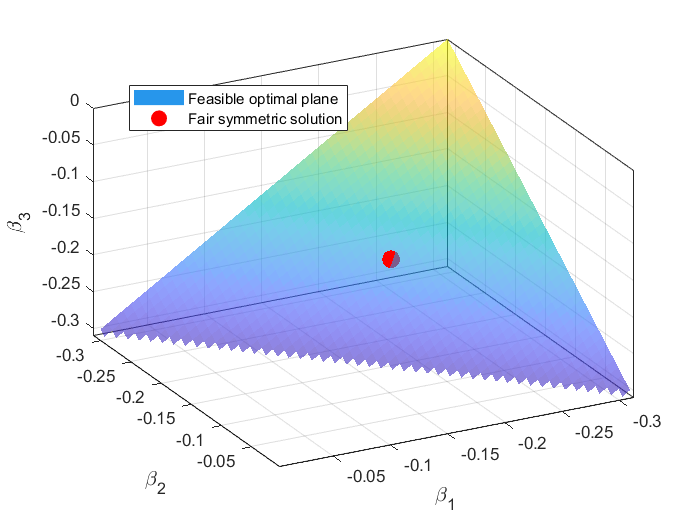
\includegraphics[width=1\linewidth]{figures/risk_seek_sol.png}
    \caption{Feasible risk seeking Pareto allocations (with $n=3$).}
    \label{fig:beta_rs}
\end{figure}

\subsection{Analytical and Centralized Nash Solutions}

We compare the following prescribed bidding configurations:
\begin{itemize}
    \item Coalition bidding strategy \eqref{eq:alpha_1} (if all agree to join); 
    \item Risk seeking Pareto-optimal Nash strategy \eqref{eq:alpha_i}, that is,
\begin{subequations}
\begin{align}
\alpha_1^*
&=
\frac{(1+4a_2\beta_1)\eta_1^{-1}}
{4\left(1+a_2(\beta_1+\beta_2+\beta_3)\right)},
\\[6pt]
\alpha_2^*
&=
\frac{(1+4a_2\beta_2)\eta_2^{-1}}
{4\left(1+a_2(\beta_1+\beta_2+\beta_3)\right)},
\\[6pt]
\alpha_3^*
&=
\frac{(1+4a_2\beta_3)\eta_3^{-1}}
{4\left(1+a_2(\beta_1+\beta_2+\beta_3)\right)},
\end{align}
\label{eq:3p}
\end{subequations}
which has many risk aware choices for $\beta_i$. 
\item Risk neutral Nash strategy (which is given by \eqref{eq:3p} with $\beta_i=0$). 
\end{itemize}
It follows from Lemma~1 that, if all operators cooperate and 
adopt the coalition strategy, their bids are $\alpha^*=\frac{1}{2}$ (with $\beta^*=0$), which yields $f(\boldsymbol{\alpha}^*)=\frac{1}{2}$, $g^C(\boldsymbol{\alpha}^*) = 22{,}500$\,MW$^2$, and the total profit of $\Pi^C = 10{,}800$\,\$/hr. This serves as the upper bound for the collective profit.

It follows from \eqref{eq:3p} with $\beta_i=0$ that the risk neutral Nash bidding strategies are $\boldsymbol{\alpha}^* =(\alpha_1^*, \alpha_2^*, \alpha_3^*) = (0.625, 0.75, 0.9375)$, which results in $f(\boldsymbol{\alpha}^*)=0.75$, $g(\boldsymbol{\alpha}^*)=16{,}875$\,MW$^2$, and the total profit $\Pi^{RN} = 9{,}675$\,\$/hr. In this case, the collective profit is $10.42\%$ below that under the coalition solution. On the other hand risk seeking Pareto-optimal Nash bidding strategies in \eqref{eq:3p} allow coordinated coefficient assignments that differ across controllers as long as constraint \eqref{eq:beta_sum_condition} is satisfied. Admissible choices of $\beta_i$ form the region shown in Figure~\ref{fig:beta_rs}. For the coordinated design assigning the same coefficient to every controller, we know from \eqref{eq:beta_sum_condition} that $\beta_i^* = -\frac{5}{3} $ (equivalently $\beta_i^{\prime *} = a_2\beta_i^* = -\frac{1}{6}$), which yields $\boldsymbol{\alpha}^*=(0.4167, 0.5000, 0.6250)$, resulting in $f(\boldsymbol{\alpha}^*)=0.5$, $g(\boldsymbol{\alpha}^*)=22{,}500$\,MW$^2$, and the total profit $\Pi^{ERS} = 10{,}800$\,\$/hr. This risk seeking Pareto-optimal Nash solution fully recovers the total profit under the coalition strategy.
 
\begin{table}[hbt!]
\centering
\caption{Bidding Strategy Performance: Scenario 1 \\($n=3$, $x^o=(120,100,80)$\,MW, with ERS yielding no overbidding)}
\label{tab:comparison}
\resizebox{\columnwidth}{!}{%
\begin{tabular}{|l|c|c|c|c|}
\hline
Strategy & $\boldsymbol{\alpha}^*$ & $f(\boldsymbol{\alpha}^*)$ & $g(\boldsymbol{\alpha}^*)$ in MW$^2$ & $\Pi$ in \$/hr \\
\hline
Coalition       & $(0.50,\;0.50,\;0.50)$ & $0.50$ & $22{,}500$ & $10{,}800$ \\
RN Nash         & $(0.63,\;0.75,\;0.94)$ & $0.75$ & $16{,}875$ & $\phantom{0}9{,}675$ \\
ERS Nash  & $(0.42,\;0.50,\;0.63)$ & $0.50$ & $22{,}500$ & $10{,}800$ \\
Algorithm~1 & $(0.42,\;0.50,\;0.63)$ & $0.50$ & $22{,}500$ & $10{,}800$ \\
\hline
\end{tabular}}
\end{table}


\begin{comment}
\begin{figure}[hbt!]
    \centering
    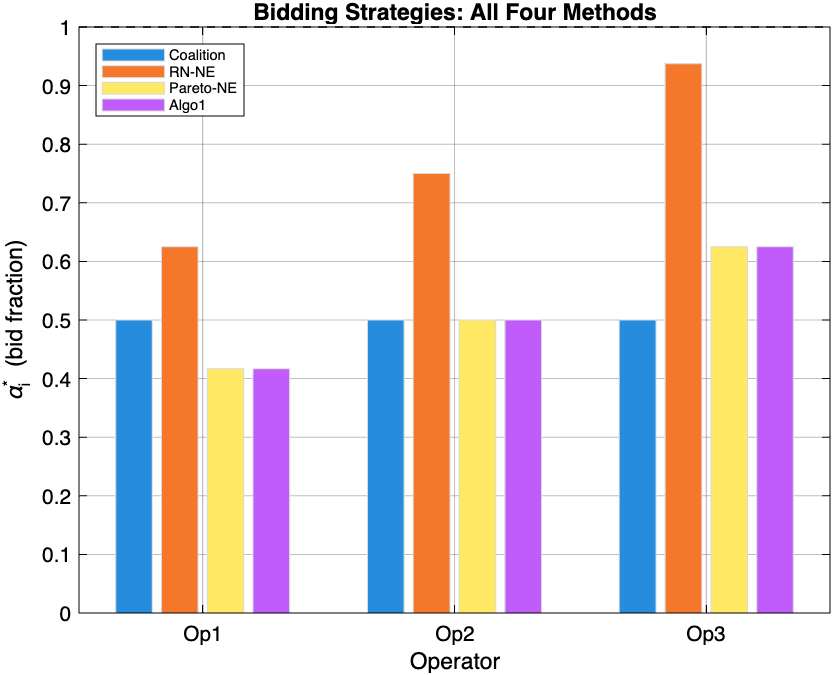
\includegraphics[width=1\linewidth]{figures/algorithm1_comp_alpha_s1.png}
    \caption{Bidding strategies $\alpha_i^*$ for all four strategies.}
    \label{fig:algo1_comp_alpha}
\end{figure}

\begin{figure}[hbt!]
    \centering
    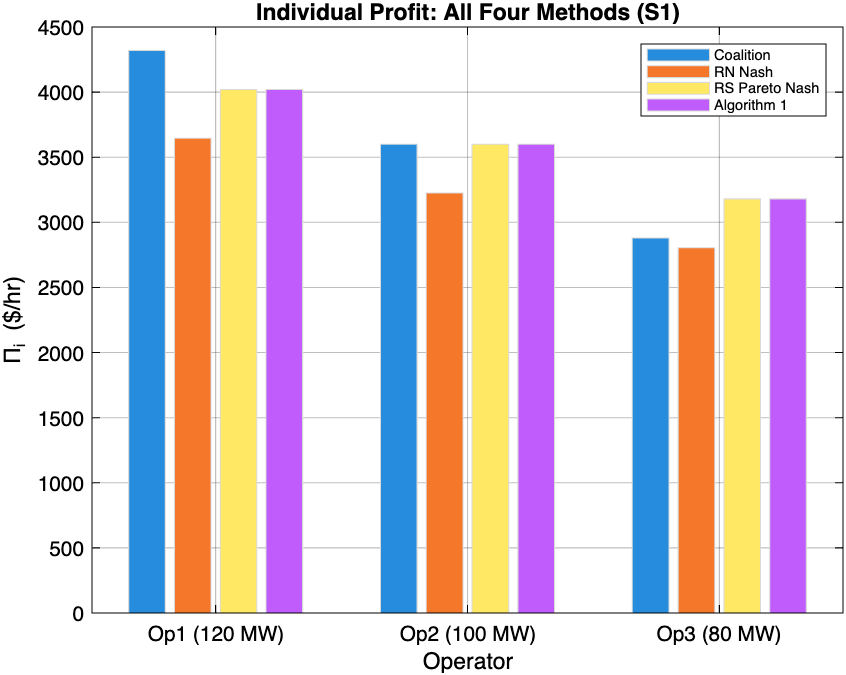
\includegraphics[width=1\linewidth]{figures/algorithm1_comp_profit_s1.png}
    \caption{Individual profits $\Pi_i$ for all four strategies (Scenario~1).}
    \label{fig:algo1_comp_profit}
\end{figure}
\end{comment}

\begin{figure}[H]
    \centering
    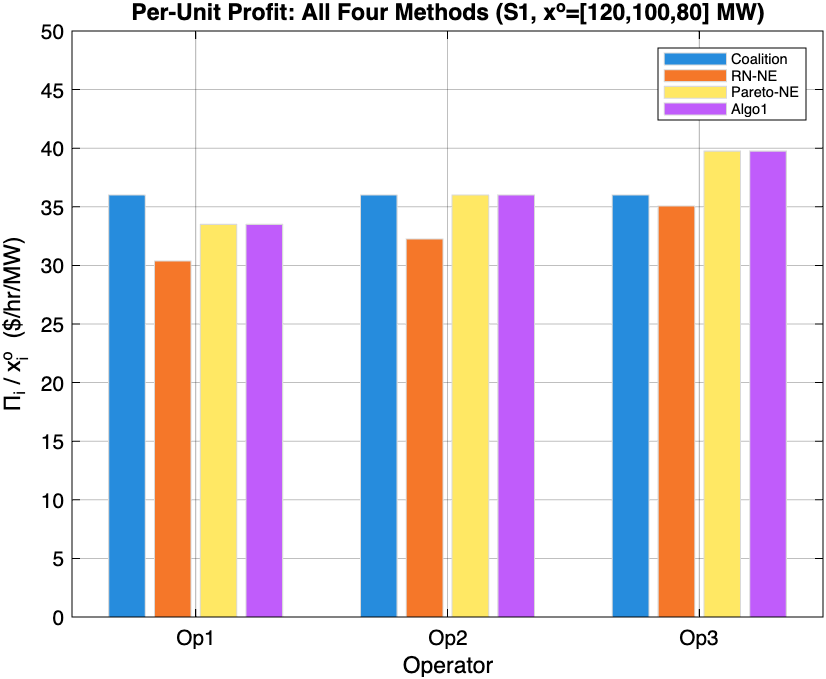
\includegraphics[width=1\linewidth]{figures/algorithm1_comp_profit_perunit_s1.png}
    \caption{Per-unit profit $\Pi_i/x_i^o$ (\$/hr/MW) for all four strategies (Scenario~1, with ERS yielding no overbidding)}
    \label{fig:algo1_comp_profit_perunit_s1}
\end{figure}

Table~\ref{tab:comparison} reports the centralized ERS values also recovered by Algorithm~\ref{alg:dist_risk_aware}: with public $n=3$ and decoded $X=300$\,MW, each operator submits $q_i=50$\,MW and keeps its bidding fraction local. The resulting aggregate profit equals the coalition benchmark. The comparison of profit allocations is separate from validation of the masking protocol below.

Figure~\ref{fig:algo1_comp_profit_perunit_s1} compares 
per-unit profits under the four different strategies. Specifically, we see that all the operators share the same per-unit profit under the coalition strategy and the total profit is maximized; that all the operators achieve lower profits under the risk neutral Nash strategy, with the higher-capacity operator(s) suffering more reduction; and that equal risk seeking Nash strategy (either centralized or distributed) achieves Pareto-optimal performance (the same as the coalition strategy) collectively, with the total profit being maximized (to the same value as the coalition solution) and with the lower-capacity operator(s) gaining more profit enhancement. Indeed, all the operators benefit from adopting an equal risk seeking Nash strategy, albeit non-uniformly. These are comparisons of prescribed configurations with ERS coefficient $\beta'=-\tfrac{1}{6}$; the following subsection examines alternative coordinated configurations.

\subsection{Unequal Risk Levels}

Table~\ref{tab:alpha_pi_summary} compares equal risk seeking (ERS) Nash strategy outcome versus unequal risk seeking (URS) Nash strategies' outcomes for scenario 1 (S1). In this comparison, ERS S1 serves as the baseline, and URS S1-A and S1-B are alternative coordinated coefficient configurations. Each row is evaluated with its coefficients fixed, rather than as a unilateral owner deviation. ERS S1 is based on equal risk seeking level of $\boldsymbol{\beta}'=(-\tfrac{1}{6},\,-\tfrac{1}{6},\,-\tfrac{1}{6})$, URS S1-A corresponds to $\boldsymbol{\beta}'=(-0.10,\,-0.17,\,-0.23)$, and  URS S1-B uses $\boldsymbol{\beta}'=(-0.23,\,-0.17,\,-0.10)$. The risk seeking levels of both
URS S1-A and URS S1-B satisfy condition $\sum_i\beta_i'=-\tfrac{1}{2}$, that is, equality \eqref{eq:beta_sum_condition} in Theorem 2. As a result, URS S1-A and URS S1-B achieve the same Pareto-optimal total profit $\Pi$ as ERS S1 does.


\begin{table}[hbt!]
\centering
\caption{Unequal Risk Levels: Scenario 1 \\ ($n=3$, $x^o=(120,100,80)$\,MW)}
\label{tab:alpha_pi_summary}
\resizebox{\columnwidth}{!}{%
\begin{tabular}{|l|c|c|c|}
\hline
Allocation & $\boldsymbol{\alpha}^*$ & $\Pi_i/x_i^o$\, in \$/(hr$\cdot$MW) & $\Pi$\, in \$/hr \\
\hline
ERS S1             & $(0.417,\,0.500,\,0.625)$ & $(33.5,\,36.0,\,39.8)$ & $10{,}800$ \\
URS S1-A           & $(0.750,\,0.480,\,0.150)$ & $(43.5,\,35.4,\,25.5)$ & $10{,}800$ \\
URS S1-B & $(0.100,\,0.480,\,1.125)$ & $(24.0,\,35.4,\,54.8)$ & $10{,}800$ \\
URS S1-C & $(0.100,\,0.480,\,1.000)$ & $(24.2,\,36.4,\,53.0)$ & $10{,}784$ \\
URS S1-D           & $(0.292,\,0.350,\,1.000)$ & $(29.8,\,31.5,\,51.0)$ & $10{,}800$ \\
\hline
\end{tabular}}
\end{table}

While $\Pi$ is optimized, there are substantial disparities among the values of $\Pi_i$ under URS S1-A and URS S1-B. This is because different coefficients assigned to the controllers push some of their bidding values substantially away from coalition bidding values or ERS bidding values. These allocation differences motivate comparing equal and unequal controller designs; they do not establish which design an owner would select strategically.

URS strategy S1-B also pushes operator 3's bid above $1$, which is an overbidding case. Capping $\alpha_3^*$ at $1$ renders URS strategy S1-C and while simple for operator 3 to implement, it is no longer Pareto optimal. URS strategy S1-D restores Pareto optimality by re-calculating $\alpha_i^*$ according to the spirit of Corollary 5. More on overbidding, its impact, and its removal are delineated in the next subsection.

\subsection{Causes and Removal of Overbidding}

The Scenario~2 and~3 tables use ``Legacy distributed'' for the original unmasked saturated calculation. The retained plots label that same calculation ``Algorithm 1''; this legacy label does not refer to the masked Algorithm~\ref{alg:dist_risk_aware} in Section~V. These figures compare allocations only and provide no evidence for the new privacy guarantee.

Overbid occurs when $\alpha_i^*>1$, i.e., an operator (or several) commits more to the day-ahead market than his/her forecast capacity $x_i^o$ and thereby exposes itself to a real-time shortfall. Inequalities \eqref{eq:eta_0} and \eqref{eq:overbid_bound} provide explicit conditions on no overbidding for RN and ERS strategies, respectively. Among the two bidding strategies, the RN strategy is more susceptible than ERS to overbidding. The following discussion reveals that overbidding is mostly a structural consequence of forecast capacity dispersion: a low-forecast operator is forced to inflate its bid in order to claim its Pareto-optimal profit share from the markets. Nonetheless, Table \ref{tab:alpha_pi_summary} also shows that a poor choice of risk level (in the sense of being either too high or too low when compared to the choices by others) may also induce overbidding. In any case, overbidding can be outlawed by the grid operator, and renewable operators can respond by implementing the clamped RN and ERS strategies in corollaries 4 and 5, respectively. 

\begin{table}[hbt!]
\centering
\caption{Bidding Strategy Performance: Scenario 2 \\ ($n=3$, $x^o=(120,100,30)$\,MW, with ERS yielding $|\Omega_{\rm ERS}|=1$)}
\label{tab:ers_compare_s2}
\resizebox{\columnwidth}{!}{%
\begin{tabular}{|l|c|c|c|}
\hline
Strategy & $\boldsymbol{\alpha}^*$ & $\Pi_i/x_i^o$\, in \$/(hr$\cdot$MW) & $\Pi$\, in \$/hr \\
\hline
Coalition                & $(0.500,\,0.500,\,0.500)$ & $(43.5,\,43.5,\,43.5)$ & $10{,}875$ \\
RN Nash - unclamped  & $(0.521,\,0.625,\,2.083)$ & $(37.5,\,38.8,\,57.0)$ & $10{,}094$ \\
RN Nash - clamped    & $(0.611,\,0.733,\,1.000)$ & $(40.0,\,41.8,\,45.7)$ & $10{,}341$ \\
ERS Nash - unclamped  & $(0.347,\,0.417,\,1.389)$ & $(39.7,\,41.4,\,65.7)$ & $10{,}875$ \\
ERS Nash - clamped & $(0.396,\,0.475,\,1.000)$ & $(40.9,\,42.9,\,56.0)$ & $10{,}875$ \\
Legacy distributed & $(0.396,\,0.475,\,1.000)$ & $(40.9,\,42.9,\,56.0)$ & $10{,}875$ \\
\hline
\end{tabular}}
\end{table}

\begin{comment}
\begin{figure}[hbt!]
    \centering
    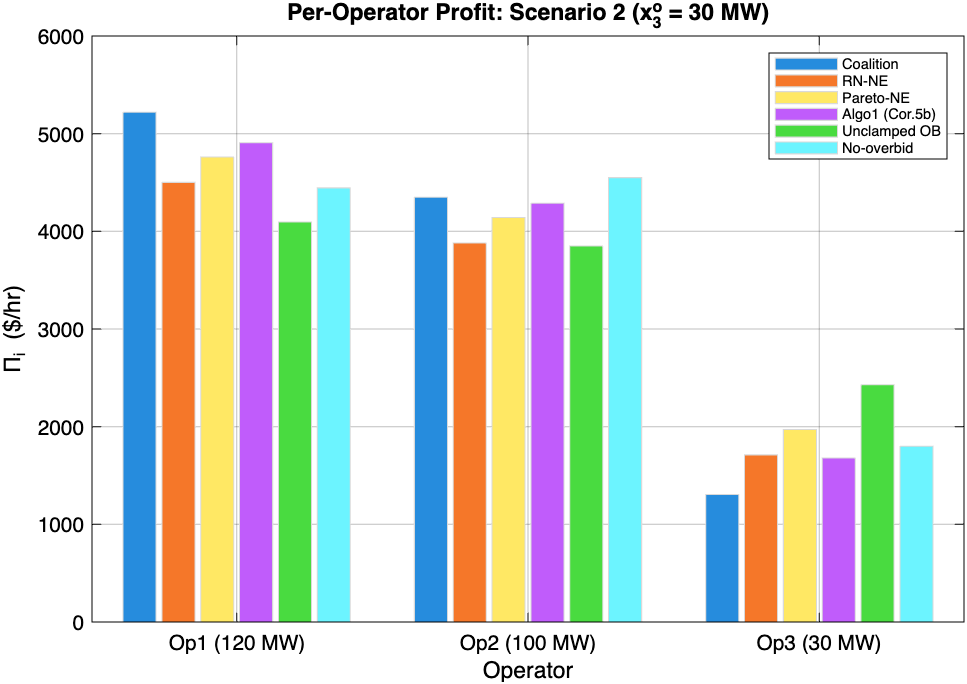
\includegraphics[width=1\linewidth]{figures/algorithm1_overbid_profit_s2.png}
    \caption{Per-operator profit $\Pi_i$ under Scenario~2. Coalition and the legacy saturated calculation attain the maximum profit with deliverable bids; the feasible risk neutral strategy leaves a gap, and the unclamped optimum is physically infeasible.}
    \label{fig:algo1_overbid_profit}
\end{figure}
\end{comment}

\begin{figure}[hbt!]
    \centering
    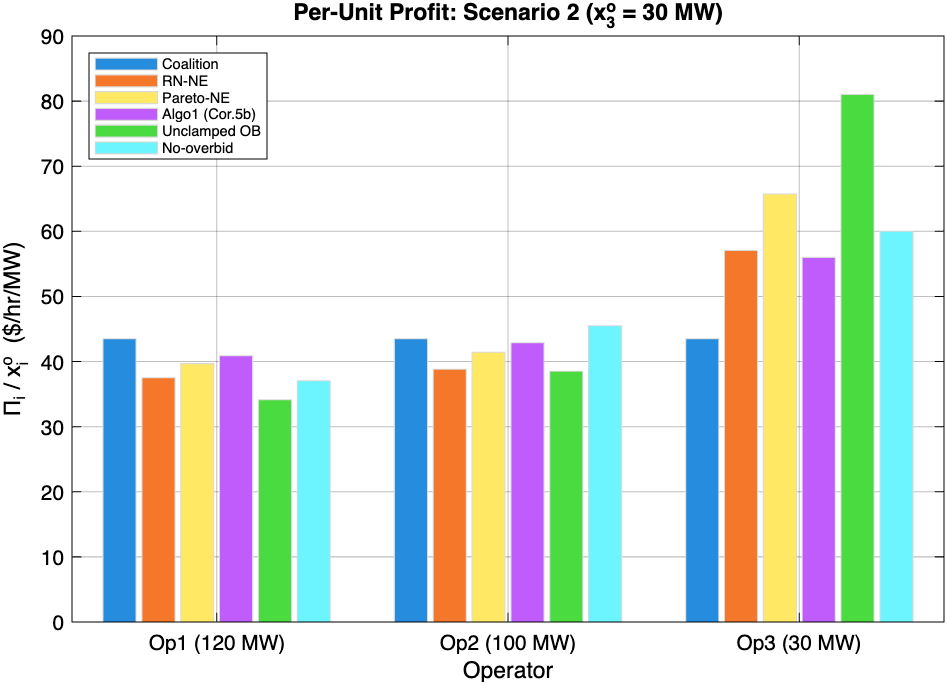
\includegraphics[width=1\linewidth]{figures/algorithm1_overbid_profit_perunit_s2.png}
    \caption{Per-unit profit $\Pi_i/x_i^o$ under Scenario~2; the plot label ``Algorithm 1'' denotes the legacy unmasked calculation}
    \label{fig:algo1_overbid_profit_perunit}
\end{figure}

As Scenario 2, consider forecast vector $\boldsymbol{\eta}=(0.48,\,0.40,\,0.12)$ which is more dispersed than scenario 1's. The corresponding results under coalition strategy, RN strategy, and ERS strategy are summarized into  
Table~\ref{tab:ers_compare_s2}. Since $\eta_3<\frac16$, operator~3 is forced to overbid in order to claim its Pareto shares, should overbidding be allowed; otherwise, the clamped versions are used. It is clear that the coalition strategy provides not only the maximum total profit but also equal unit profit. Should full cooperation be out of reach, each renewable operator can adopt Nash strategies. In the risk neutral setting, overbidding by operator 3 increases its payoff, but the total payoff is lower, which reveals the unfair distortion of overbidding; and the clamped RN strategy not only reduces the distortion but also increases the total payoff. In the equal risk seeking setting, the total payoff becomes Pareto optimal and equals to that under the coalition strategy, but the unclamped ERS strategy yields higher per-unit payoff for those who overbid, while clamped ERS strategy narrows the differences in per-unit payoffs. These observations are also confirmed by the plots of per-unit profits in Fig.~\ref{fig:algo1_overbid_profit_perunit}. 



\begin{table}[hbt!]
\centering
\caption{Bidding Strategy Performance: Scenario 3 \\ ($n=3$, $x^o=(210,45,45)$\,MW, with ERS yielding $|\Omega_{\rm ERS}|=2$)}
\label{tab:ers_compare_s3}
\resizebox{\columnwidth}{!}{%
\begin{tabular}{|l|c|c|c|}
\hline
Strategy & $\boldsymbol{\alpha}^*$ & $\Pi_i/x_i^o$\, in \$/(hr$\cdot$MW) & $\Pi$\, in \$/hr \\
\hline
Coalition                & $(0.500,\,0.500,\,0.500)$ & $(36.0,\,36.0,\,36.0)$ & $10{,}800$ \\
RN Nash - unclamped & $(0.357,\,1.667,\,1.667)$ & $(26.4,\,46.0,\,46.0)$ & $\phantom{0}9{,}675$ \\
RN Nash - clamped    & $(0.500,\,1.000,\,1.000)$ & $(31.5,\,42.0,\,42.0)$ & $10{,}395$ \\
ERS Nash - unclamped  & $(0.238,\,1.111,\,1.111)$ & $(28.1,\,54.3,\,54.3)$ & $10{,}800$ \\
ERS Nash - clamped & $(0.286,\,1.000,\,1.000)$ & $(29.6,\,51.0,\,51.0)$ & $10{,}800$ \\
Legacy distributed & $(0.286,\,1.000,\,1.000)$ & $(29.6,\,51.0,\,51.0)$ & $10{,}800$ \\
\hline
\end{tabular}}
\end{table}

Scenario 3 involves the forecast capacity vector $\boldsymbol{\eta}=(0.70,\,0.15,\,0.15)$, which has even more spread than the previous two scenarios. Because of $\eta_2,\eta_3<\frac16$, both operators~2 and~3 intend to overbid unless their RN and ERS strategies are clamped. Table~\ref{tab:ers_compare_s3} and Fig.~\ref{fig:algo1_overbid_profit_perunit_s3} show the same patterns as those in scenario~2. 

\begin{comment}
\begin{figure}[hbt!]
    \centering
    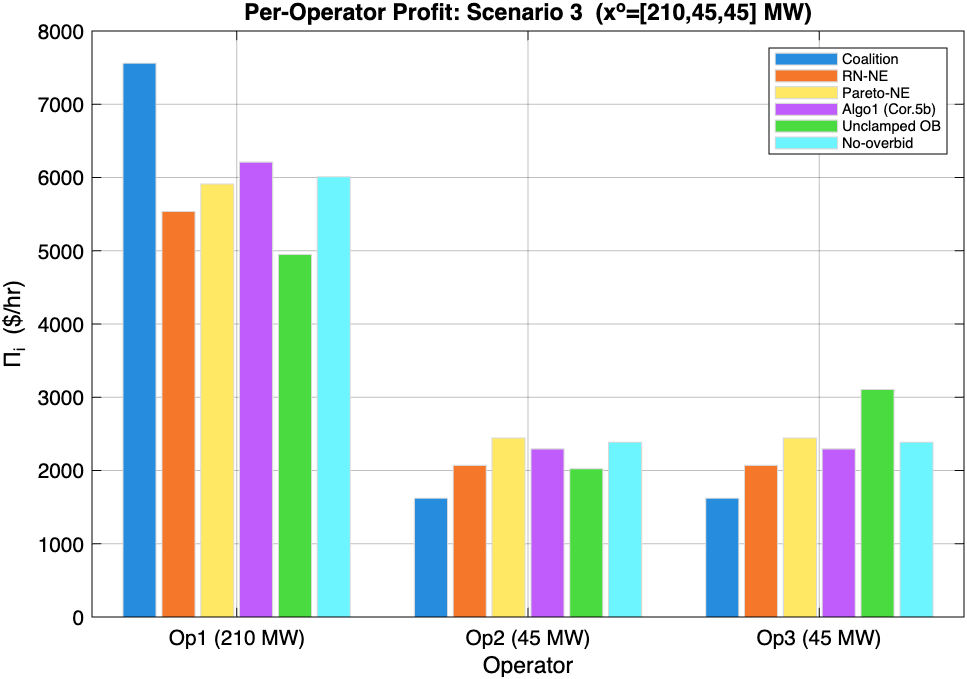
\includegraphics[width=1\linewidth]{figures/algorithm1_overbid_profit_s3.png}
    \caption{Per-operator profit $\Pi_i$ under Scenario~3. Coalition and the legacy saturated calculation attain $\Pi=10{,}800$\,\$/hr; operator~1 alone absorbs the bid adjustment for the two saturated operators.}
    \label{fig:algo1_overbid_profit_s3}
\end{figure}
\end{comment}

\begin{figure}[hbt!]
    \centering
    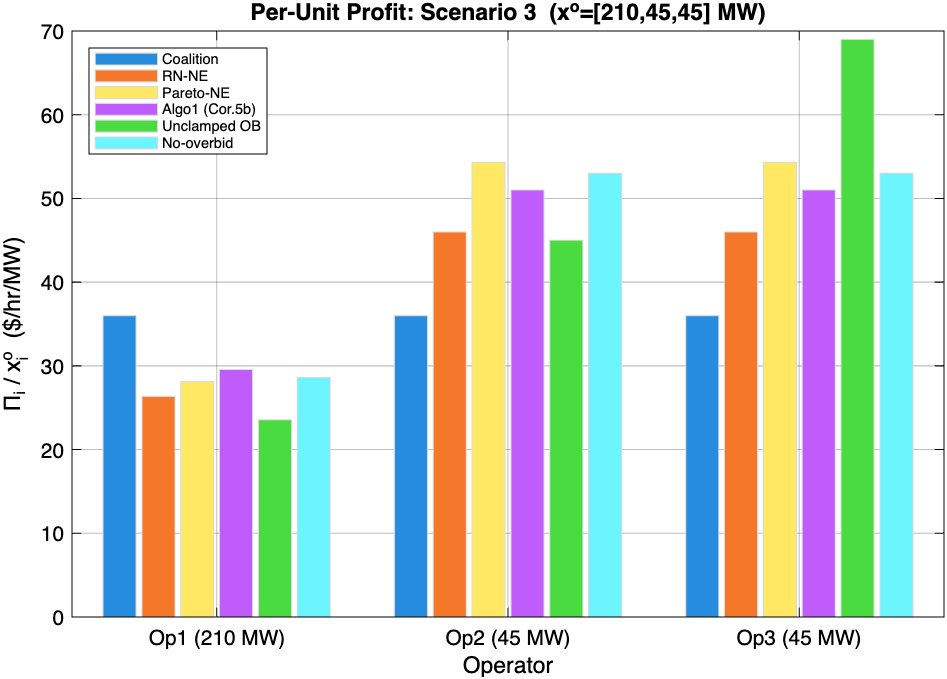
\includegraphics[width=1\linewidth]{figures/algorithm1_overbid_profit_perunit_s3.png}
    \caption{Per-unit profit $\Pi_i/x_i^o$ under Scenario~3; the plot label ``Algorithm 1'' denotes the legacy unmasked calculation}
    \label{fig:algo1_overbid_profit_perunit_s3}
\end{figure}




Across the three scenarios, several general conclusions emerge:
\begin{itemize}
\item In the reported comparisons, the coalition configuration attains the maximum aggregate expected profit and equal per-unit profit. These allocation properties do not establish owner preferences or willingness to participate.
\item Relative to the coalition configuration, the reported RN and ERS bidding equilibria allocate greater per-unit profit to smaller operators and less to larger operators. ERS retains the maximum aggregate expected profit, whereas RN yields a lower total.
\item Overbidding in both RN and ERS settings would distort the per-unit profit more toward smaller market participants who would overbid. Unequal RS strategies would do the same for those who are more risk seeking and/or become overbidding. These saturated numerical comparisons concern profit allocations; they do not establish forecast privacy.  
\end{itemize}

\subsection{Masked Implementation and Communication}

For Scenario~1, a triangle mask graph, $\Delta=1$\,MW, $B=120$, $p=1009$, and reproducible test seed $20261120$ give masked inputs $(43,244,13)$. At $k_*=37$, exact rational arithmetic gives maximum scaled consensus error $0.01374$ (rounded upward), below the certified bound $0.19223<1/4$. All nodes recover $X=300$\,MW and $q_i=50$\,MW, preserving the centralized ERS bids and profits. An exhaustive check over all $7^3$ triangle-mask assignments for inputs $(1,1,2)$ and $(1,2,1)$ gives identical view distributions, including for a utility colluding with operator~1; removing the remaining honest edge makes the views distinguishable. These finite checks illustrate Proposition~2 and its connectivity requirement; they do not replace its proof. The reproducible masks are public test data, not production secrets.

For $G_c=K_{1,n}$ and $h=1/(n+1)$, $\rho=n/(n+1)$ for $n\geq2$. Hence the sufficient decoding budget is $O(n\log(m^{3/2}p))$ rounds with a fixed arithmetic-error margin, with $2n$ directed scalar transmissions per round. Masking adds one private field element per edge of $G_m$ per run. The graph must remain connected after removal of the colluding operators; a complete mask graph tolerates any coalition leaving at least two honest operators. Thus communication and the required precision depend on $n$ and $p$; size-independent convergence is not claimed.

Additional deterministic checks are summarized in Table~\ref{tab:mask_validation}. All cases use public $B=120$, $\Delta=1$\,MW, a cycle mask graph, a star consensus graph, and $h=1/(n+1)$. Forecasts for $n>3$ are reproducibly generated integers in $[80,120]$ using seed $20261117+n$; the $n=3$ forecasts are those of Scenario~1. Each decoding budget satisfies the conservative ideal-arithmetic bound $m^{3/2}(p-1)\rho^{k_*}<1/4$. Every node recovers the correct sum and the centralized ERS quantities. The three-operator run uses exact rational arithmetic. Larger runs use binary64 arithmetic and are empirical correctness checks, not certified roundoff guarantees or timing benchmarks. The corresponding logical consensus transmission counts are $2nk_*$; secure-channel establishment and cryptographic byte overhead are excluded.

\begin{table}[hbt]
\centering
\caption{Deterministic masked-consensus checks}
\label{tab:mask_validation}
\begin{tabular}{rrrrr}
\hline
$n$ & $p$ & $k_*$ & Ideal bound & Observed error\\
\hline
3 & 1009 & 37 & 0.19223 & 0.01373\\
10 & 1201 & 127 & 0.24233 & 0.03421\\
50 & 6007 & 808 & 0.24604 & 0.01858\\
100 & 12007 & 1780 & 0.24765 & 0.01301\\
\hline
\end{tabular}
\end{table}

Here ``observed error'' is $\max_i|m\psi_i(k_*)-\sum_jy_j|$, before integer rounding and modular reduction. A second exact-rational three-operator run, with seed $20261121$, gives $y=(903,687,728)$ and $\sum_i y_i=2318=300+2(1009)$; rounding followed by reduction modulo $1009$ again recovers $300$. This explicitly checks modular wraparound. In the exhaustive $p=7$, $B=2$ test, the $343$ equally likely triangle-mask assignments give $49$ public masked vectors, each with multiplicity $7$, for either input. Including operator~1's input and its incident masks in the adversarial view also gives identical distributions. When removing the honest edge disconnects the noncolluding operators, their individual inputs can instead be recovered. These checks distinguish protocol correctness, finite illustrations of privacy, and the general proof in Proposition~2.

The accompanying Python validation script records public test masks, input vectors, seeds, decoding results, and exact-arithmetic error fractions. It is a reference validation model; it does not implement confidential channels or production cryptographic randomness.

% Legacy unmasked experiments below are excluded from the paper and privacy claims.
\begin{comment}
To assess the robustness of the overbidding analysis with respect to initial risk profiles, the outer-loop coordination of $\beta_i'$ is evaluated under six heterogeneous starting points: risk neutral ($\beta_i'(0)=0$), uniform risk seeking ($\beta_i'(0)=-1$), uniform risk averse ($\beta_i'(0)=1$), and three mixed profiles. Figures~\ref{fig:mc_overbid_count} and~\ref{fig:mc_overbid_profit} show the per-operator overbidding indicator and aggregate profit comparison for each case. Operators with smaller capacity shares saturate first in every case, consistent with the threshold ordering of Remark~1. Cases where no operator overbids throughout coordination (e.g., the ERS) yield identical unclamped and clamped profit trajectories, while cases with high initial risk seeking values exhibit a transient profit gap that closes as $\sum\beta_i'$ converges to the Pareto target.

\begin{figure}[hbt!]
    \centering
    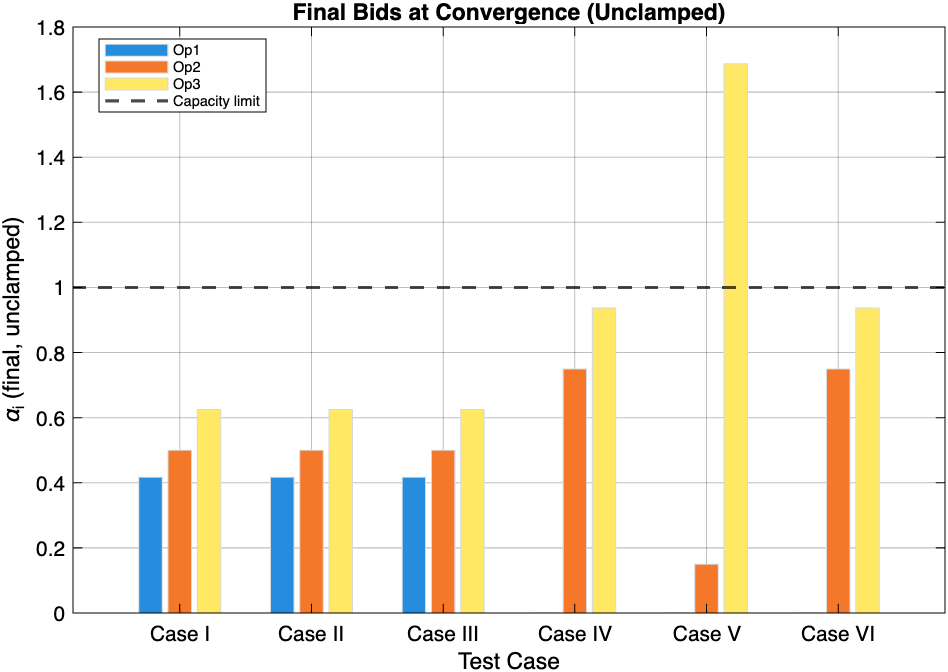
\includegraphics[width=1\linewidth]{figures/mc_overbid_count.png}
    \caption{Per-operator overbidding indicator ($\alpha_i > 1$, shown as 0/1) across six initial risk profiles. Operators with smaller capacity shares ($\eta_i$) saturate earlier in coordination, and the fraction of saturating operators (dashed) confirms the threshold ordering of Remark~1 across all cases.}
    \label{fig:mc_overbid_count}
\end{figure}

\begin{figure}[hbt!]
    \centering
    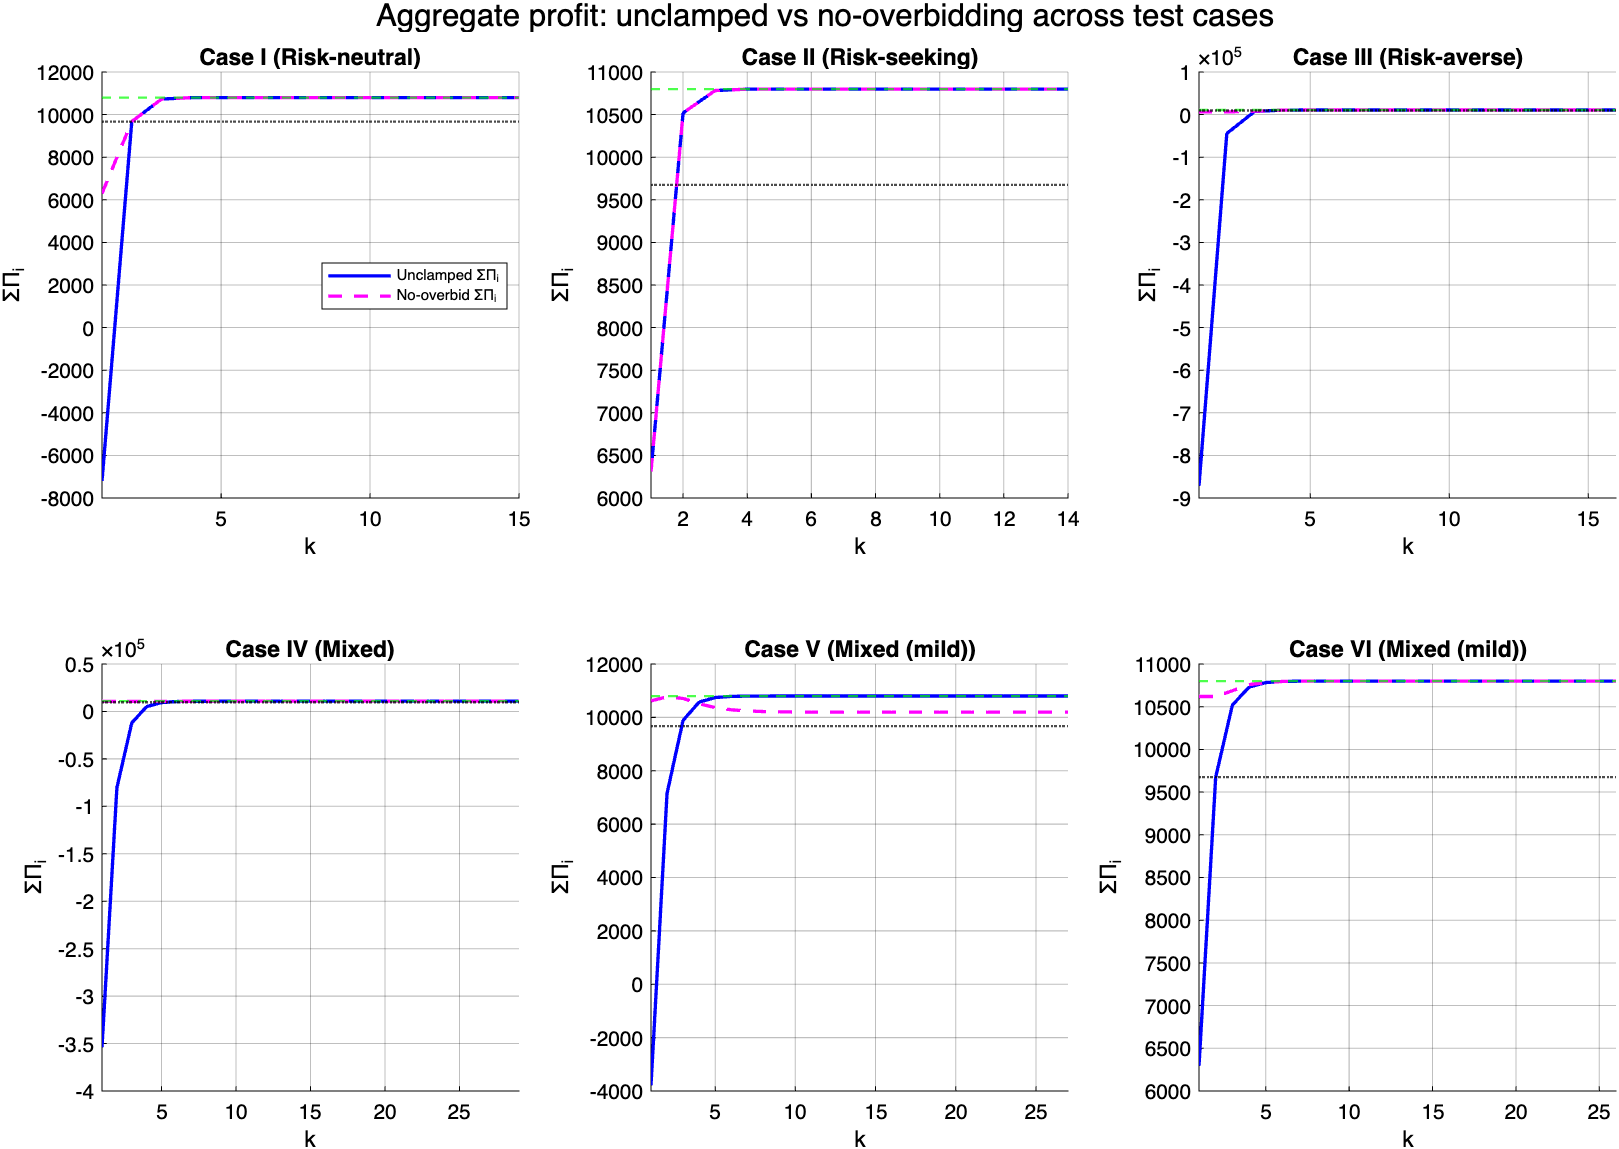
\includegraphics[width=1\linewidth]{figures/mc_overbid_profit.png}
    \caption{Aggregate profit $\sum_i\Pi_i$ under unclamped versus no-overbidding projection across six initial risk profiles. The profit gap is case-dependent and governed by the number of saturating operators; cases with no overbidding show identical trajectories. All cases converge to the Pareto-optimal profit level as coordination proceeds.}
    \label{fig:mc_overbid_profit}
\end{figure}
\end{comment}

\begin{comment}
\subsubsection{Algorithm 2: Non-Equal Initial Risk Parameters}
Algorithm~\ref{alg:dist_risk_aware_beta_coord} is evaluated using \texttt{risk\_aware\_power\_system.m} under multiple heterogeneous initial conditions $\beta_i'(0)$. The study focuses on whether distributed coordination of the aggregate risk parameter and unclamped one-shot bidding preserve the Pareto target. Accordingly, bid/profit comparisons are reported in this subsection (after the risk-parameter coordination stage is complete).

\begin{figure}[hbt!]
    \centering
    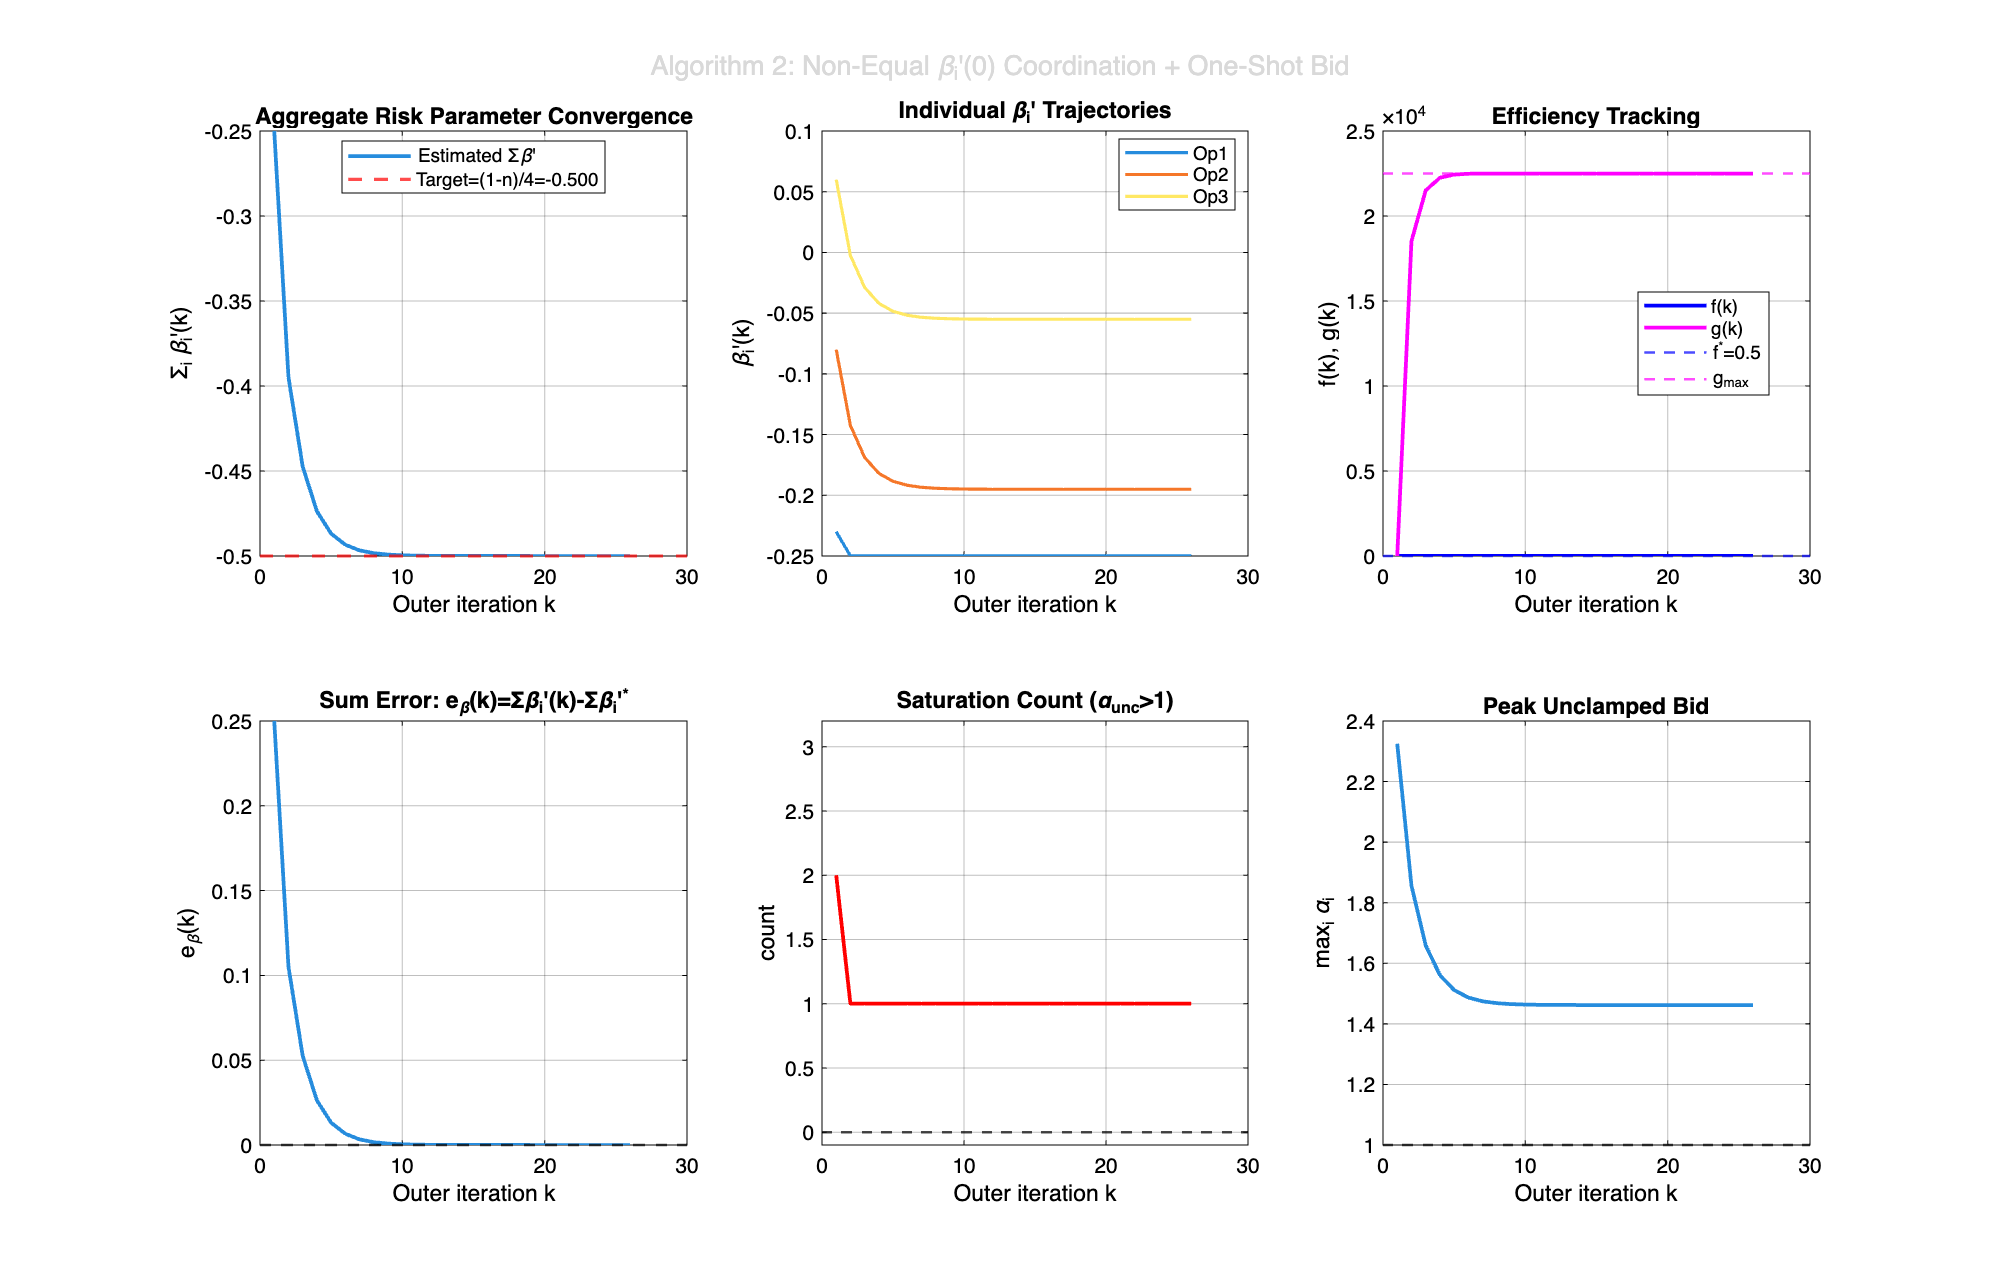
\includegraphics[width=1\linewidth]{figures/algorithm2_results.png}
    \caption{Algorithm~2 single-scenario diagnostics: convergence of $\sum\beta_i'$, individual $\beta_i'$, efficiency metrics, and saturation count.}
    \label{fig:algo2_single}
\end{figure}

\begin{figure}[hbt!]
    \centering
    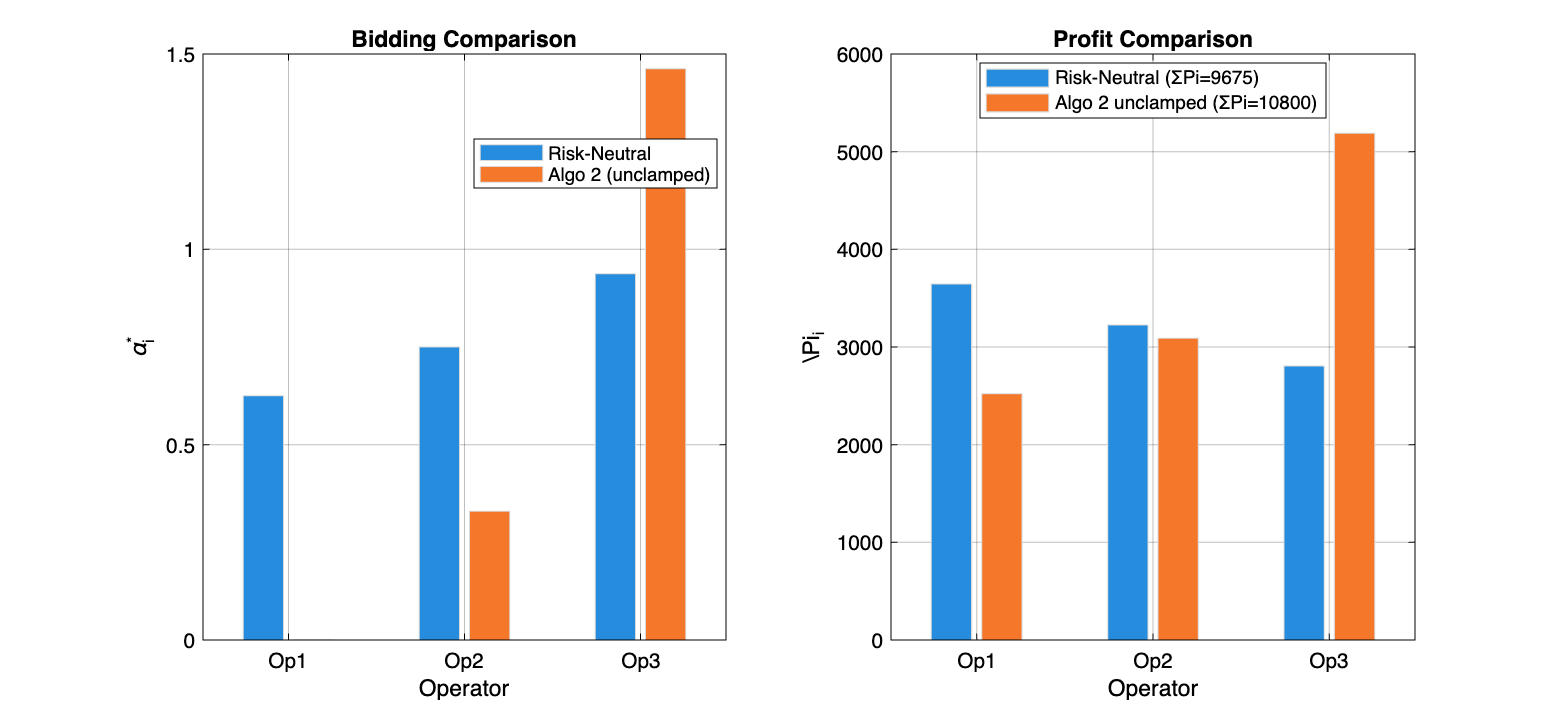
\includegraphics[width=1\linewidth]{figures/algorithm2_bidding_comparison.png}
    \caption{Algorithm~2 bidding/profit comparison under the unclamped $\alpha_i$ assumption.}
    \label{fig:algo2_bidprofit}
\end{figure}

\begin{figure}[hbt!]
    \centering
    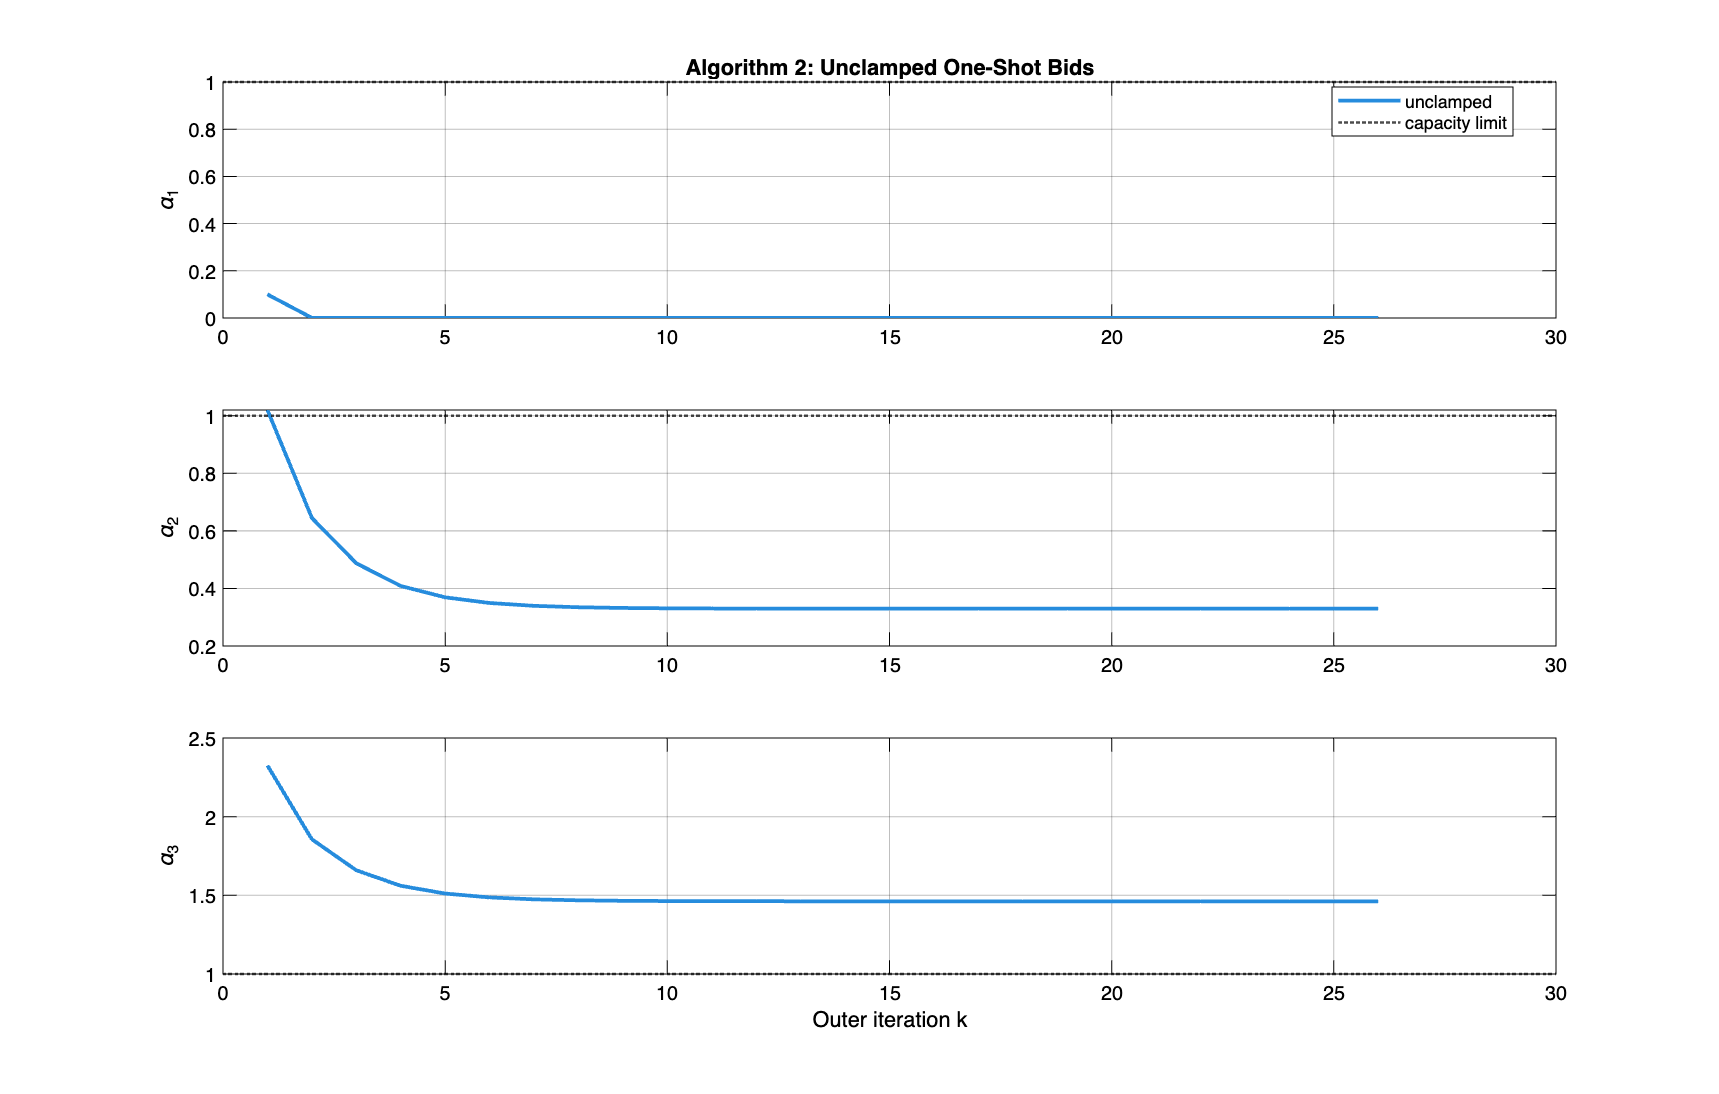
\includegraphics[width=1\linewidth]{figures/algorithm2_alpha_unclamped.png}
    \caption{Algorithm~2 one-shot bid trajectories under the unclamped $\alpha_i$ assumption, with capacity limit shown for reference.}
    \label{fig:algo2_clamp}
\end{figure}

\begin{table}[h]
\centering
\caption{Test cases with initial transformed risk parameters $\beta_i' = a_2\beta_i$}
\label{tab:test_cases}
\begin{tabular}{lcccc}
\hline
Test case & $\beta_1'$ & $\beta_2'$ & $\beta_3'$ & Risk Profile \\
\hline
I & 0 & 0 & 0 & Risk-neutral \\
II & -1 & -1 & -1 & Risk-seeking \\
III & 1 & 1 & 1 & Risk-averse \\
IV & -1 & 1 & 1 & Mixed \\
V & -0.25 & 0 & 0.20 & Mixed \\
VI & -0.25 & 0 & 0 & Mixed \\
\hline
\end{tabular}
\end{table}

\begin{figure}[hbt!]
    \centering
    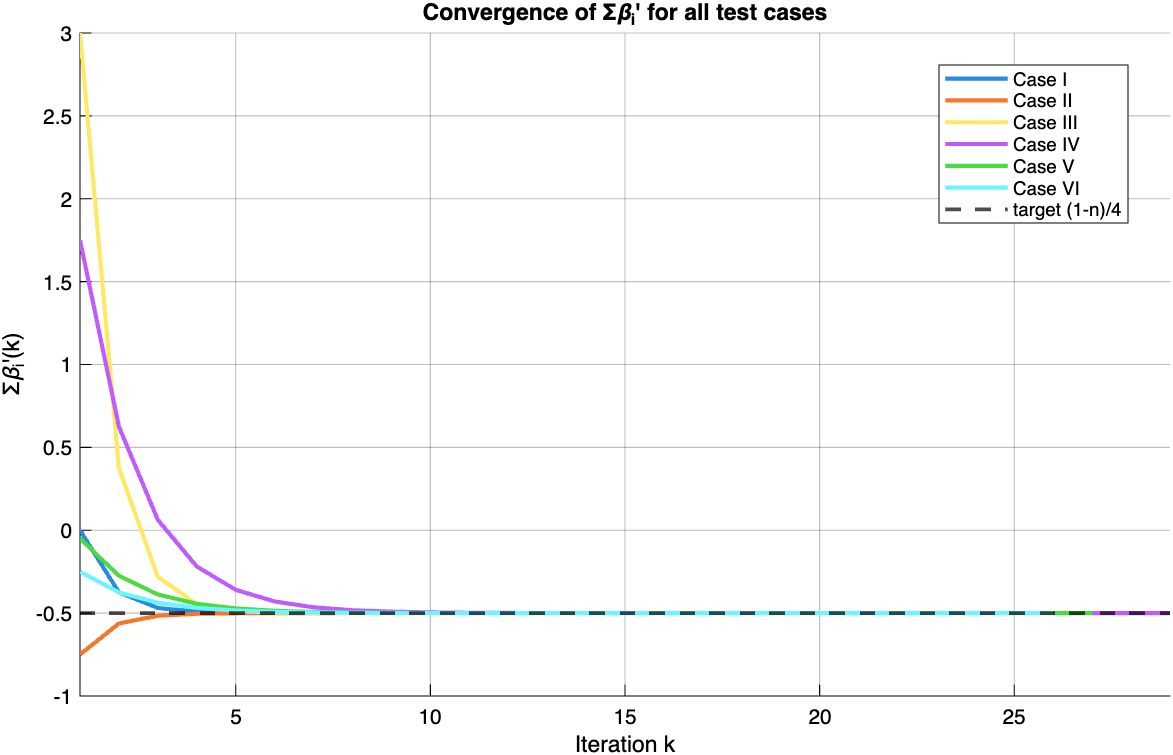
\includegraphics[width=1\linewidth]{figures/sum_beta_convergence_all_cases.png}
    \caption{Convergence of $\sum\beta_i'$ for all test cases. Each case converges to the Pareto-optimal sum $\sum\beta_i'^* = (1-n)/4 = -0.5$.}
    \label{fig:sum_beta_all}
\end{figure}

\begin{figure}[hbt!]
    \centering
    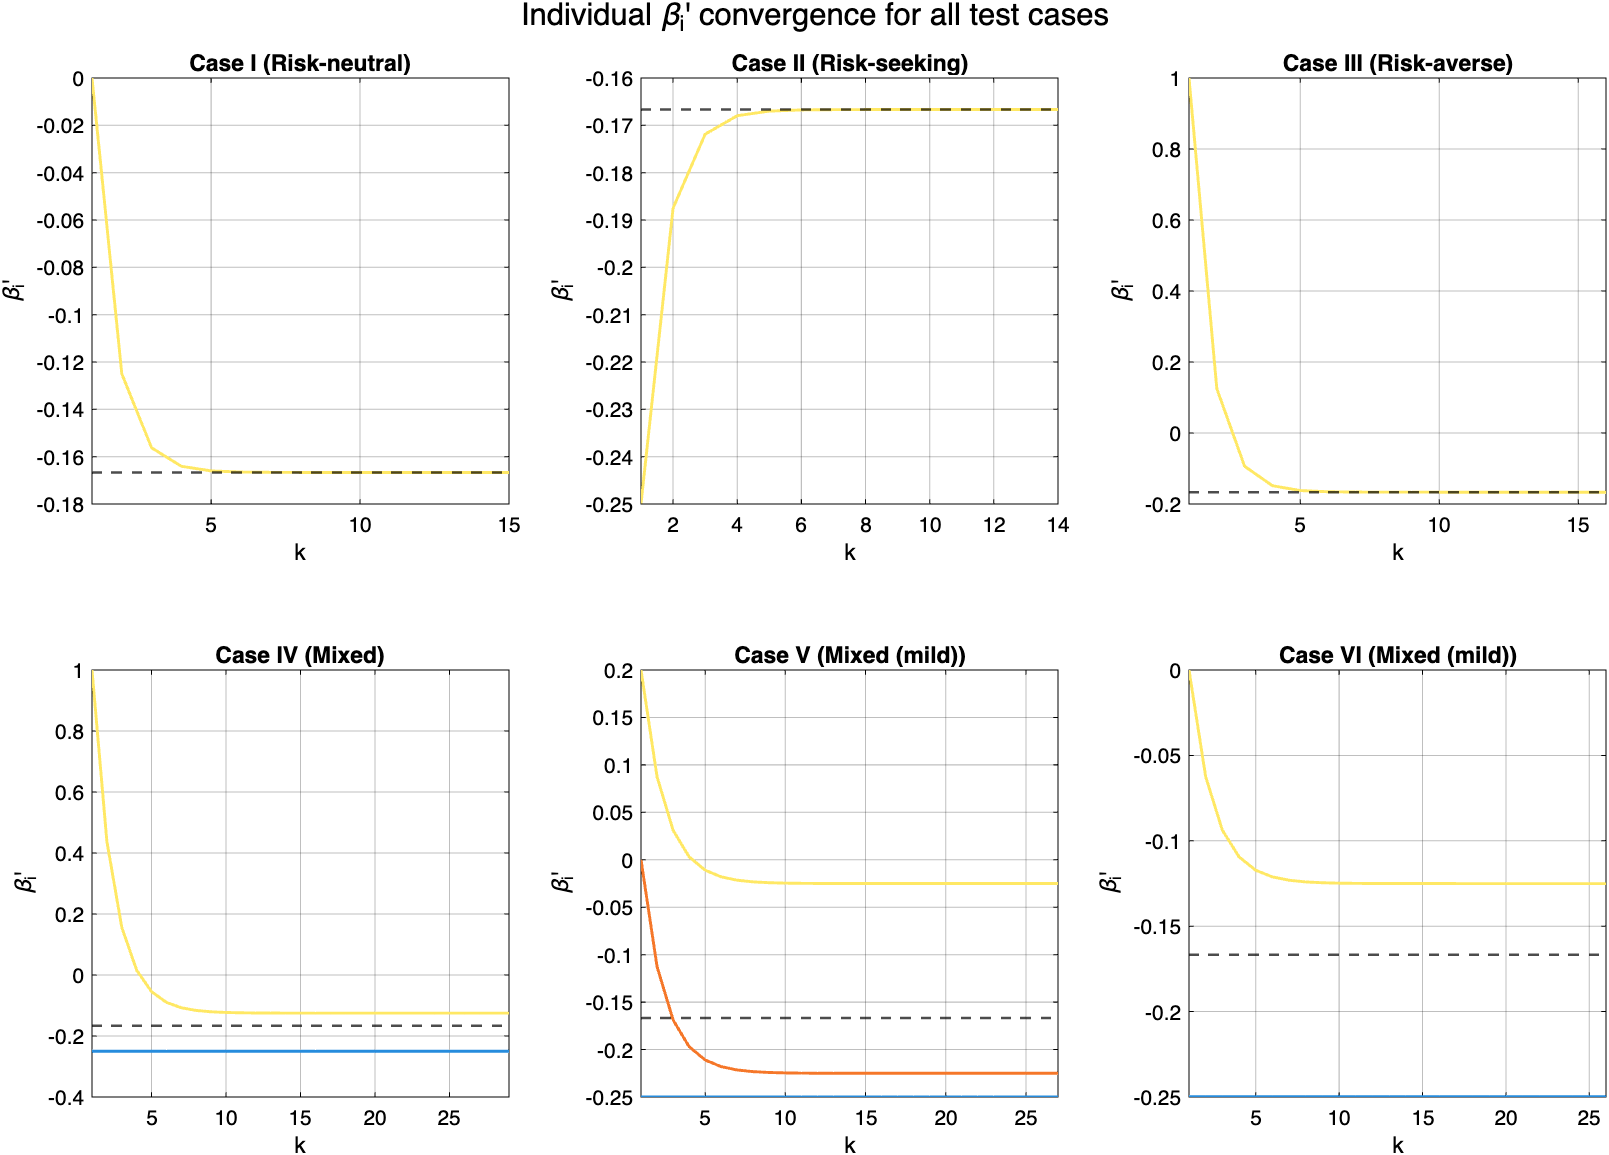
\includegraphics[width=1\linewidth]{figures/beta_individual_all_cases.png}
    \caption{Individual $\beta_i'$ convergence for each test case. Most cases achieve the Pareto-optimal sum; cases with capacity-constrained operators may converge to alternative equilibria (see Remark~1).}
    \label{fig:beta_individual}
\end{figure}

\begin{figure}[hbt!]
    \centering
    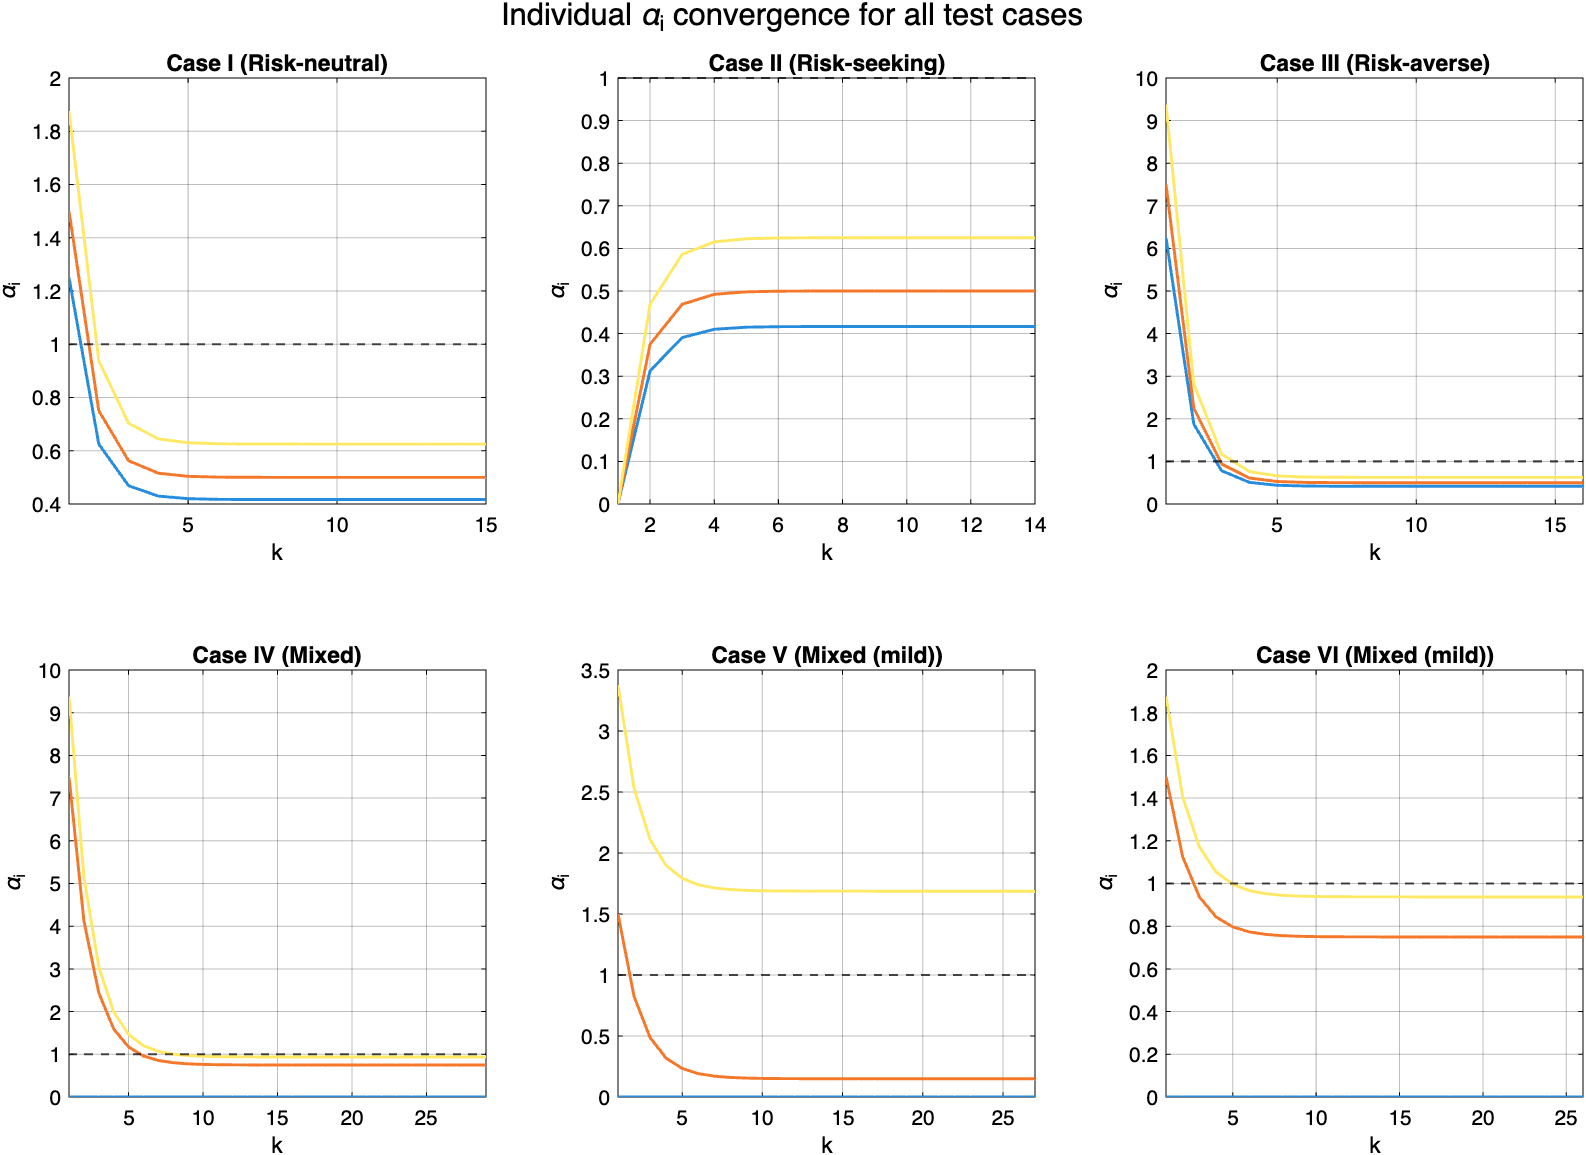
\includegraphics[width=1\linewidth]{figures/alpha_individual_all_cases.png}
    \caption{Individual $\alpha_i$ convergence for each test case. Bidding fractions adjust to achieve $f(\alpha) = 0.5$.}
    \label{fig:alpha_individual}
\end{figure}

Figure~\ref{fig:sum_beta_all} shows the convergence of the aggregate risk parameter $\sum\beta_i'$ for all test cases. Despite vastly different initial conditions ranging from risk neutral (Case~I) to risk seeking (Case~II) to risk averse (Case~III) to mixed profiles (Cases~IV--VI), most cases converge to the Pareto-optimal value $\sum\beta_i'^* = (1-n)/4 = -0.5$ as predicted by Theorem~2. For cases with unequal risk preferences where capacity constraints bind (see Remark~1), the algorithm may converge to a different $\sum\beta_i'$ while still driving $f(\alpha)$ close to $0.5$ under the unclamped-bid model. Figure~\ref{fig:beta_individual} provides a detailed view of individual $\beta_i'$ trajectories within each case, showing how operators with different initial risk preferences adapt their parameters.

Figure~\ref{fig:alpha_individual} shows the corresponding evolution of bidding fractions $\alpha_i$. As the risk parameters converge, the bidding strategies adjust to achieve $f(\alpha) = 0.5$, confirming the Nash equilibrium behavior characterized in Lemma~2. Figures~\ref{fig:algo2_single}, \ref{fig:algo2_bidprofit}, and~\ref{fig:algo2_clamp} further illustrate the single-scenario dynamics of Algorithm~2 under the unclamped-bid assumption. The impact of the risk-parameter updates on market efficiency is illustrated in Figures~\ref{fig:f_all} and~\ref{fig:S_all}, where the aggregate bidding fraction $f(\alpha)$ converges to $1/2$ and the error signal $|S|$ decreases below the convergence  for all test cases.

\begin{figure}[hbt!]
    \centering
    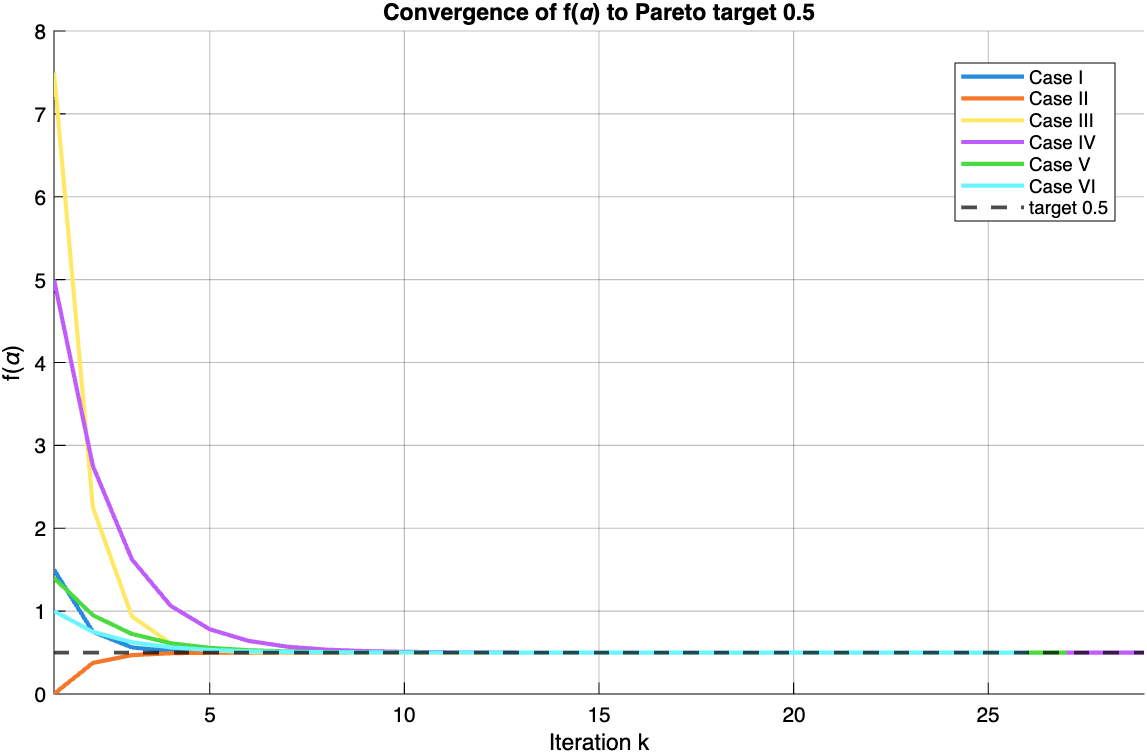
\includegraphics[width=1\linewidth]{figures/f_convergence_all_cases.png}
    \caption{Convergence of aggregate bidding fraction $f(\alpha)$ to Pareto target $0.5$ for all test cases.}
    \label{fig:f_all}
\end{figure}

\begin{figure}[hbt!]
    \centering
    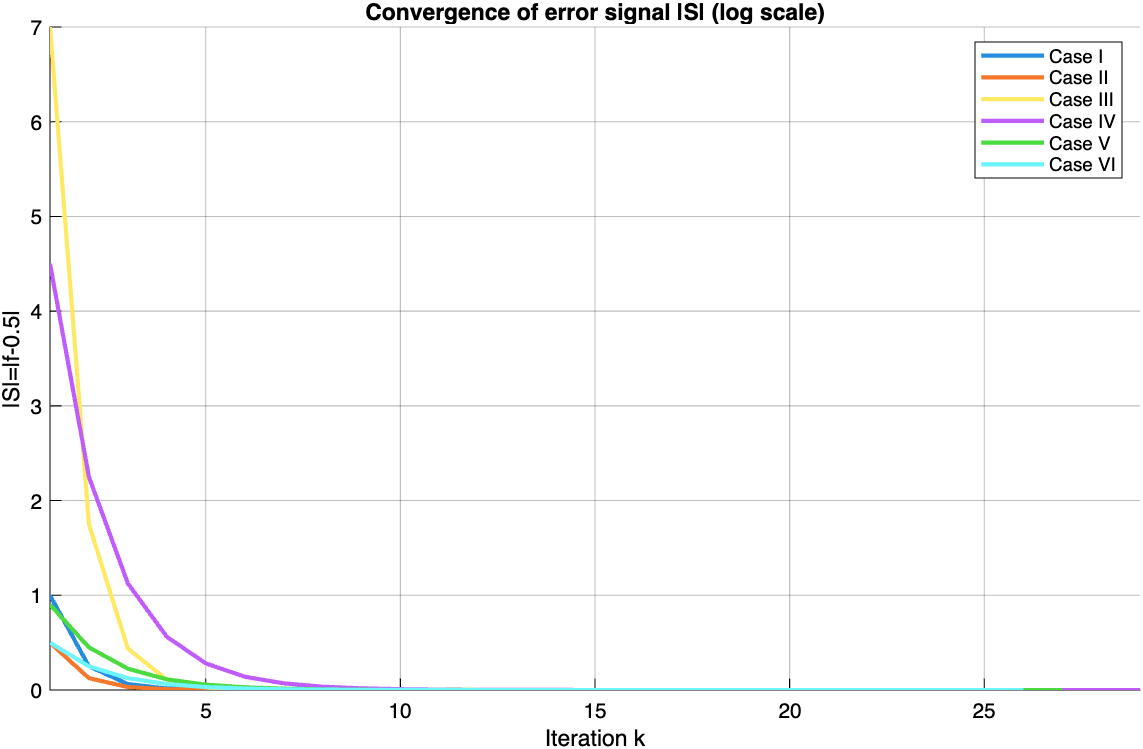
\includegraphics[width=1\linewidth]{figures/S_convergence_all_cases.png}
    \caption{Convergence of error signal $|S| = |f - 0.5|$ (log scale) for all test cases.}
    \label{fig:S_all}
\end{figure}

\begin{figure}[hbt!]
    \centering
    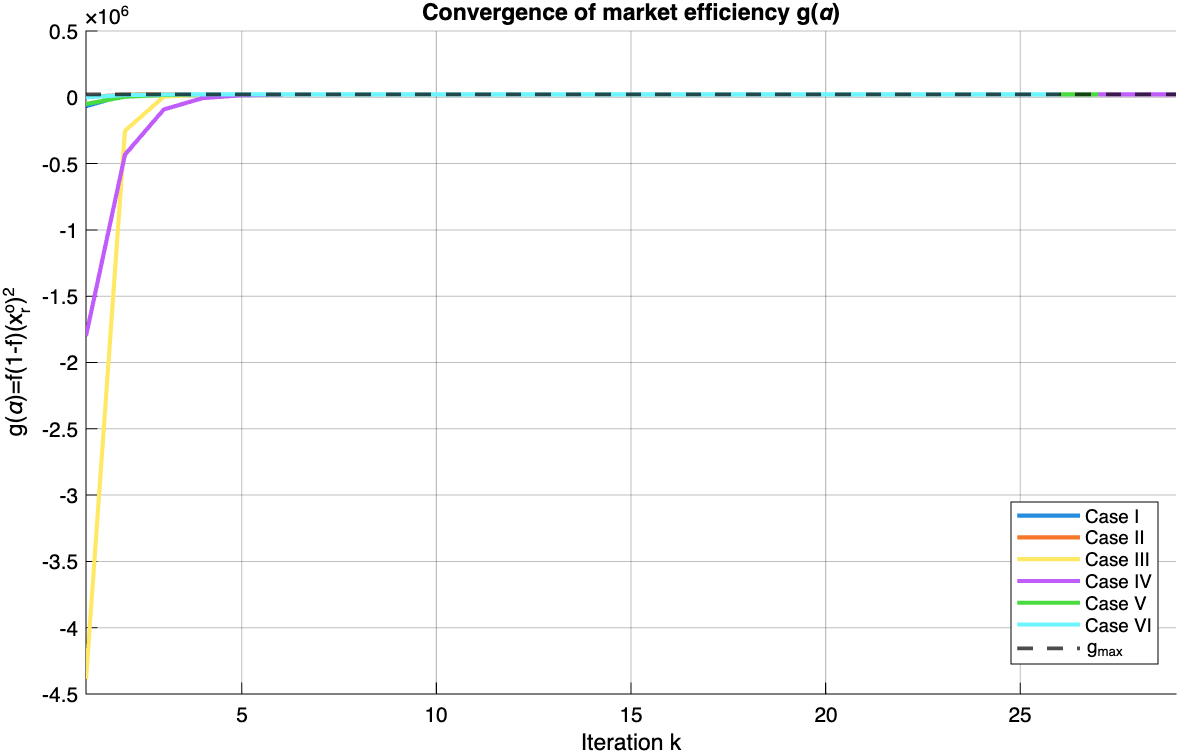
\includegraphics[width=1\linewidth]{figures/g_convergence_all_cases.png}
    \caption{Convergence of market efficiency $g(\alpha) = f(1-f)(x_r^o)^2$ to maximum value $g_{\max} = 0.25(x_r^o)^2$ for all test cases.}
    \label{fig:g_all}
\end{figure}

\begin{figure}[hbt!]
    \centering
    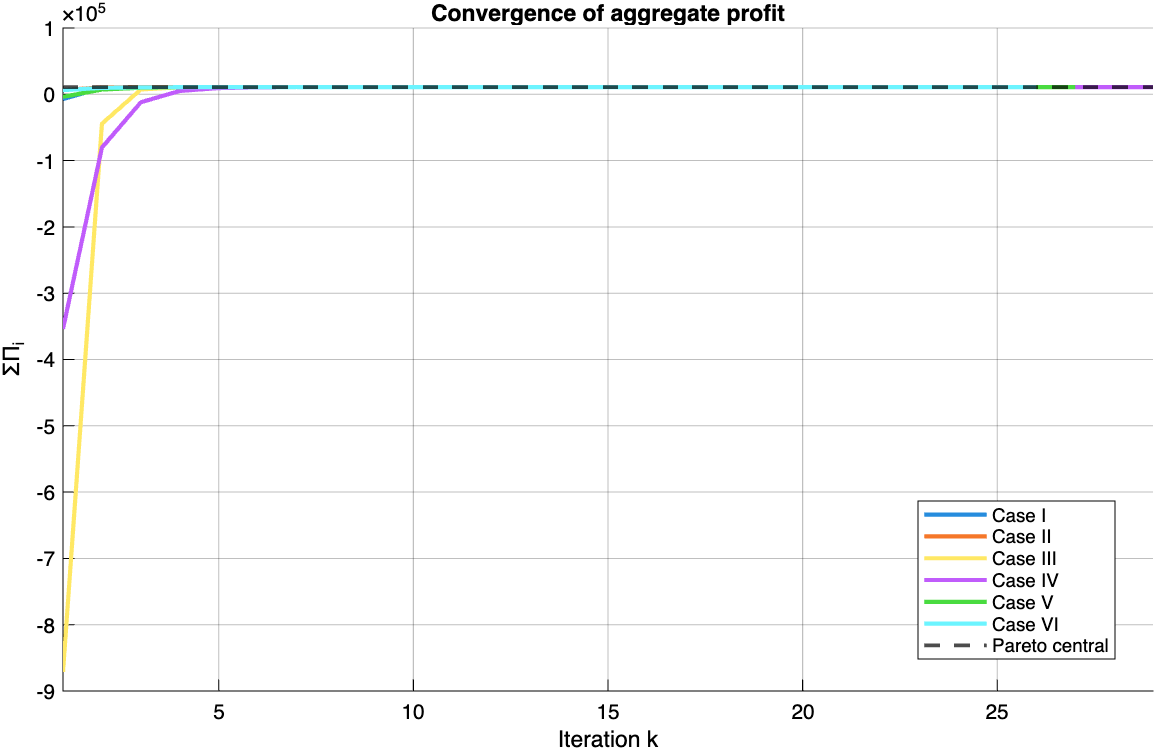
\includegraphics[width=1\linewidth]{figures/profit_convergence_all_cases.png}
    \caption{Convergence of aggregate profit $\sum\Pi_i$ for all test cases.}
    \label{fig:profit_all}
\end{figure}

Figure~\ref{fig:g_all} demonstrates that market efficiency $g(\alpha)$ converges to its maximum value $g_{\max} = 0.25(x_r^o)^2 = 22{,}500$ for all test cases, confirming that the distributed algorithm successfully achieves Pareto optimality. Figure~\ref{fig:profit_all} shows the corresponding convergence of aggregate profits $\sum\Pi_i$.

Notably, for mixed risk profiles where some operators are risk seeking while others are risk averse (e.g., Case~V), the unconstrained model can produce $\alpha_i>1$ for risk averse operators, as discussed in Remark~1. In such cases, the aggregate risk parameter $\sum\beta_i'$ may not converge exactly to $(1-n)/4$; yet the algorithm still drives $f(\alpha)$ toward $0.5$ and near-Pareto aggregate profit. This demonstrates the robustness of the distributed approach under heterogeneous risk preferences.

These results validate that the proposed distributed algorithm achieves Pareto-enhanced Nash equilibria using only local computations and minimal information exchange. Regardless of initial risk preferences, the algorithm guides all operators toward the collective optimum. In particular, the renewable operators do not require knowledge of other agents' forecasts, cost parameters, or private objectives, yet collectively achieve the same performance as a centralized optimizer. This highlights the practicality of the proposed framework for real-time electricity markets with decentralized renewable participants.
\end{comment}

\section{Conclusion}

This paper separates coordinated design of risk aware bidding controllers from the noncooperative bidding game played with their coefficients fixed. In the uncapped model, the aggregate coefficient condition identifies designs whose bidding Nash equilibrium attains the coalition benchmark for aggregate expected renewable profit. Equal risk seeking provides a symmetric coefficient choice. Masked consensus recovers its target bids exactly for encoded forecasts and limits transcript disclosure under the stated channel, connectivity, and passive-adversary assumptions. Nash optimality is evaluated using the controller objectives $J_i$; profit efficiency is evaluated using $\Pi_i$.

The unilateral-deviation analysis shows that equal risk seeking is not an equilibrium of unrestricted coefficient selection by expected-profit-maximizing owners. Implementation therefore assumes adherence to the coordinated controllers. Designing and validating a mechanism that makes adoption and continued adherence individually optimal remains a separate problem.

Further analysis is done to delineate the conditions under which renewable operators and microgrid aggregators may overbid in both risk neutral and risk seeking settings. The conditions are in terms of relative dispersion of operators' capacities. No-overbidding Pareto-optimal Nash strategies are also developed in general. And illustrative examples are included to demonstrate Pareto optimality of risk seeking Nash strategies, their no-overbidding version. The masked implementation and privacy theorem apply only to uncapped ERS. 

\bibliographystyle{IEEEtran}
\bibliography{references}

\end{document}
